% Options for packages loaded elsewhere
\PassOptionsToPackage{unicode}{hyperref}
\PassOptionsToPackage{hyphens}{url}
\PassOptionsToPackage{dvipsnames,svgnames,x11names}{xcolor}
%
\documentclass[
]{article}

\usepackage{amsmath,amssymb}
\usepackage{iftex}
\ifPDFTeX
  \usepackage[T1]{fontenc}
  \usepackage[utf8]{inputenc}
  \usepackage{textcomp} % provide euro and other symbols
\else % if luatex or xetex
  \usepackage{unicode-math}
  \defaultfontfeatures{Scale=MatchLowercase}
  \defaultfontfeatures[\rmfamily]{Ligatures=TeX,Scale=1}
\fi
\usepackage{lmodern}
\ifPDFTeX\else  
    % xetex/luatex font selection
\fi
% Use upquote if available, for straight quotes in verbatim environments
\IfFileExists{upquote.sty}{\usepackage{upquote}}{}
\IfFileExists{microtype.sty}{% use microtype if available
  \usepackage[]{microtype}
  \UseMicrotypeSet[protrusion]{basicmath} % disable protrusion for tt fonts
}{}
\makeatletter
\@ifundefined{KOMAClassName}{% if non-KOMA class
  \IfFileExists{parskip.sty}{%
    \usepackage{parskip}
  }{% else
    \setlength{\parindent}{0pt}
    \setlength{\parskip}{6pt plus 2pt minus 1pt}}
}{% if KOMA class
  \KOMAoptions{parskip=half}}
\makeatother
\usepackage{xcolor}
\setlength{\emergencystretch}{3em} % prevent overfull lines
\setcounter{secnumdepth}{-\maxdimen} % remove section numbering
% Make \paragraph and \subparagraph free-standing
\makeatletter
\ifx\paragraph\undefined\else
  \let\oldparagraph\paragraph
  \renewcommand{\paragraph}{
    \@ifstar
      \xxxParagraphStar
      \xxxParagraphNoStar
  }
  \newcommand{\xxxParagraphStar}[1]{\oldparagraph*{#1}\mbox{}}
  \newcommand{\xxxParagraphNoStar}[1]{\oldparagraph{#1}\mbox{}}
\fi
\ifx\subparagraph\undefined\else
  \let\oldsubparagraph\subparagraph
  \renewcommand{\subparagraph}{
    \@ifstar
      \xxxSubParagraphStar
      \xxxSubParagraphNoStar
  }
  \newcommand{\xxxSubParagraphStar}[1]{\oldsubparagraph*{#1}\mbox{}}
  \newcommand{\xxxSubParagraphNoStar}[1]{\oldsubparagraph{#1}\mbox{}}
\fi
\makeatother


\providecommand{\tightlist}{%
  \setlength{\itemsep}{0pt}\setlength{\parskip}{0pt}}\usepackage{longtable,booktabs,array}
\usepackage{calc} % for calculating minipage widths
% Correct order of tables after \paragraph or \subparagraph
\usepackage{etoolbox}
\makeatletter
\patchcmd\longtable{\par}{\if@noskipsec\mbox{}\fi\par}{}{}
\makeatother
% Allow footnotes in longtable head/foot
\IfFileExists{footnotehyper.sty}{\usepackage{footnotehyper}}{\usepackage{footnote}}
\makesavenoteenv{longtable}
\usepackage{graphicx}
\makeatletter
\newsavebox\pandoc@box
\newcommand*\pandocbounded[1]{% scales image to fit in text height/width
  \sbox\pandoc@box{#1}%
  \Gscale@div\@tempa{\textheight}{\dimexpr\ht\pandoc@box+\dp\pandoc@box\relax}%
  \Gscale@div\@tempb{\linewidth}{\wd\pandoc@box}%
  \ifdim\@tempb\p@<\@tempa\p@\let\@tempa\@tempb\fi% select the smaller of both
  \ifdim\@tempa\p@<\p@\scalebox{\@tempa}{\usebox\pandoc@box}%
  \else\usebox{\pandoc@box}%
  \fi%
}
% Set default figure placement to htbp
\def\fps@figure{htbp}
\makeatother
% definitions for citeproc citations
\NewDocumentCommand\citeproctext{}{}
\NewDocumentCommand\citeproc{mm}{%
  \begingroup\def\citeproctext{#2}\cite{#1}\endgroup}
\makeatletter
 % allow citations to break across lines
 \let\@cite@ofmt\@firstofone
 % avoid brackets around text for \cite:
 \def\@biblabel#1{}
 \def\@cite#1#2{{#1\if@tempswa , #2\fi}}
\makeatother
\newlength{\cslhangindent}
\setlength{\cslhangindent}{1.5em}
\newlength{\csllabelwidth}
\setlength{\csllabelwidth}{3em}
\newenvironment{CSLReferences}[2] % #1 hanging-indent, #2 entry-spacing
 {\begin{list}{}{%
  \setlength{\itemindent}{0pt}
  \setlength{\leftmargin}{0pt}
  \setlength{\parsep}{0pt}
  % turn on hanging indent if param 1 is 1
  \ifodd #1
   \setlength{\leftmargin}{\cslhangindent}
   \setlength{\itemindent}{-1\cslhangindent}
  \fi
  % set entry spacing
  \setlength{\itemsep}{#2\baselineskip}}}
 {\end{list}}
\usepackage{calc}
\newcommand{\CSLBlock}[1]{\hfill\break\parbox[t]{\linewidth}{\strut\ignorespaces#1\strut}}
\newcommand{\CSLLeftMargin}[1]{\parbox[t]{\csllabelwidth}{\strut#1\strut}}
\newcommand{\CSLRightInline}[1]{\parbox[t]{\linewidth - \csllabelwidth}{\strut#1\strut}}
\newcommand{\CSLIndent}[1]{\hspace{\cslhangindent}#1}

% Author metadata shared by the arXiv and BRM editions.
\makeatletter
\renewcommand{\maketitle}{%
  \begin{center}
  {\Large\bfseries \@title\par}\vspace{1em}
  Aleksandar Tomašević\textsuperscript{1}, Hudson Golino\textsuperscript{2}, and
  Alexander P. Christensen\textsuperscript{3}\par\vspace{0.5em}
  {\small
  \textsuperscript{1}Institute of Physics Belgrade, University of Belgrade\par
  \textsuperscript{2}Department of Psychology, University of Virginia\par
  \textsuperscript{3}Department of Psychology and Human Development, Peabody College, Vanderbilt University\par}
  \end{center}
  \noindent Correspondence: Aleksandar Tomašević, Institute of Physics Belgrade,
  University of Belgrade, Pregrevica 118, 11080 Belgrade, Serbia.
  Telephone: +381 (0)11 37 13 000. Email: \href{mailto:atomasevic@ipb.ac.rs}{atomasevic@ipb.ac.rs}.\par
  \noindent ORCID: Aleksandar Tomašević 0000-0003-4863-6051;
  Hudson Golino 0000-0002-1601-1447;
  Alexander P. Christensen 0000-0002-9798-7037.\par
  \vspace{1em}
}
\makeatother
% BRM review layout: page numbers at the upper right, including the title page.
\usepackage{fancyhdr}
\setlength{\headheight}{14pt}
\pagestyle{fancy}
\fancyhf{}
\fancyhead[R]{\thepage}
\renewcommand{\headrulewidth}{0pt}
\fancypagestyle{plain}{\fancyhf{}\fancyhead[R]{\thepage}\renewcommand{\headrulewidth}{0pt}}
\let\submissiontitle\maketitle
\renewcommand{\maketitle}{\submissiontitle\clearpage}
\AtEndEnvironment{abstract}{\clearpage}
\raggedbottom
\usepackage{setspace}
\usepackage{placeins}
\usepackage{float}
\usepackage{hyperref}
\hypersetup{colorlinks=true, linkcolor=blue, urlcolor=blue, citecolor=blue}
\usepackage[margin=1in]{geometry}
\usepackage{lineno}
\usepackage{amsmath}
\usepackage{booktabs}
\usepackage{pdflscape}
\doublespacing
\linenumbers
\makeatletter
\@ifpackageloaded{caption}{}{\usepackage{caption}}
\AtBeginDocument{%
\ifdefined\contentsname
  \renewcommand*\contentsname{Table of contents}
\else
  \newcommand\contentsname{Table of contents}
\fi
\ifdefined\listfigurename
  \renewcommand*\listfigurename{List of Figures}
\else
  \newcommand\listfigurename{List of Figures}
\fi
\ifdefined\listtablename
  \renewcommand*\listtablename{List of Tables}
\else
  \newcommand\listtablename{List of Tables}
\fi
\ifdefined\figurename
  \renewcommand*\figurename{Figure}
\else
  \newcommand\figurename{Figure}
\fi
\ifdefined\tablename
  \renewcommand*\tablename{Table}
\else
  \newcommand\tablename{Table}
\fi
}
\@ifpackageloaded{float}{}{\usepackage{float}}
\floatstyle{ruled}
\@ifundefined{c@chapter}{\newfloat{codelisting}{h}{lop}}{\newfloat{codelisting}{h}{lop}[chapter]}
\floatname{codelisting}{Listing}
\newcommand*\listoflistings{\listof{codelisting}{List of Listings}}
\makeatother
\makeatletter
\makeatother
\makeatletter
\@ifpackageloaded{caption}{}{\usepackage{caption}}
\@ifpackageloaded{subcaption}{}{\usepackage{subcaption}}
\makeatother

\usepackage{bookmark}

\IfFileExists{xurl.sty}{\usepackage{xurl}}{} % add URL line breaks if available
\urlstyle{same} % disable monospaced font for URLs
\hypersetup{
  pdftitle={Supplementary material: A Latent Oscillator Measurement Model to Simulate Emotional-Expression Score Dynamics in Video},
  pdfauthor={Aleksandar Tomašević; Hudson Golino; Alexander P. Christensen},
  pdfkeywords={classifier scores, simulation, dimensional recovery,
compositional data, dynamic networks},
  colorlinks=true,
  linkcolor={blue},
  filecolor={Maroon},
  citecolor={Blue},
  urlcolor={Blue},
  pdfcreator={LaTeX via pandoc}}


\title{Supplementary material: A Latent Oscillator Measurement Model to
Simulate Emotional-Expression Score Dynamics in Video}
\author{Aleksandar Tomašević \and Hudson Golino \and Alexander P.
Christensen}
\date{}

\begin{document}
\maketitle


Appendices A--C accompany the main manuscript. Equation numbering
continues from the main manuscript.

\setcounter{equation}{2}
\setcounter{table}{0}
\renewcommand{\thetable}{A\arabic{table}}
\setcounter{figure}{0}
\renewcommand{\thefigure}{A\arabic{figure}}

\section{Appendix A: Complete Specification of
LOMM}\label{appendix-a-complete-specification-of-lomm}

This appendix gives the formal LOMM specification behind the conceptual
account in the main text. It is intended for readers who want to
reimplement the generator or examine its assumptions and identification
limits.

\subsection{A.1 The Latent Transition}\label{a.1-the-latent-transition}

The transition below advances the latent level and velocity over one
observation interval while holding the acceleration input constant. The
matrix \(\boldsymbol\Phi_f(\Delta)\) describes how the current state
evolves, and \(\boldsymbol\Gamma_f(\Delta)\) describes how the input
changes that state. For the oscillator in Equation 1 of the main
manuscript, these are

\[
\boldsymbol{\Phi}_f(\Delta)=\exp(\mathbf{A}_f\Delta),
\qquad
\mathbf{A}_f=
\begin{bmatrix}
0 & 1 \\
\eta_f & \zeta_f
\end{bmatrix}
\qquad
\text{and}
\qquad
\boldsymbol{\Gamma}_f(\Delta)=\int_0^{\Delta}\exp(\mathbf{A}_f u)\mathbf{b}\,du,
\quad
\mathbf{b}=
\begin{bmatrix}
0 \\
1
\end{bmatrix}.
\]

For the nonzero position-feedback values used in the simulation grids,
the input map has the equivalent exact form

\[
\boldsymbol{\Gamma}_f(\Delta)
=\mathbf{A}_f^{-1}\{\boldsymbol{\Phi}_f(\Delta)-\mathbf{I}_2\}\mathbf{b}.
\]

The implemented state recurrence is

\[
\begin{bmatrix}
x_{if,n+1}\\
v_{if,n+1}
\end{bmatrix}
=
\boldsymbol{\Phi}_f(\Delta)
\begin{bmatrix}
x_{if,n}\\
v_{if,n}
\end{bmatrix}
+
\boldsymbol{\Gamma}_f(\Delta)q_{if,n},
\qquad n=1,\ldots,T-1.
\]

The integral definition remains valid when \(\mathbf{A}_f\) is singular,
including \(\eta_f=0\). If a root-based closed form is used numerically,
a separate repeated-root branch is required when \(\zeta_f^2+4\eta_f\)
is close to zero.

The state components \(x_{if,n}\) and \(v_{if,n}\) are the level and its
rate of change at \(t_n\); \(\eta_f\) is position feedback, \(\zeta_f\)
is velocity feedback, and \(\sigma_{qf}\) is the standard deviation of
the acceleration input. On the interval \([t_n,t_{n+1})\) the underlying
continuous-time model is
\(\ddot{x}_{if}(t)=\eta_f x_{if}(t)+\zeta_f\dot{x}_{if}(t)+q_{if,n}\)
with \(q_{if,n}\) held constant, so \(\boldsymbol{\Phi}_f(\Delta)\)
propagates the deterministic state and \(\boldsymbol{\Gamma}_f(\Delta)\)
loads the input.

Let \(\mathbf q_{i,n}=(q_{i1,n},\ldots,q_{im,n})^\top\) and
\(\mathbf D_q=\operatorname{diag}(\sigma_{q1},\ldots,\sigma_{qm})\). The
generator draws

\[
\mathbf q_{i,n}\sim
\mathcal N_m\!\left(\mathbf 0,\mathbf D_q\mathbf R_q\mathbf D_q\right).
\]

The primary designs use \(\mathbf R_q=\mathbf I_m\). The
correlated-input sensitivity uses
\(\mathbf R_q=(1-0.15)\mathbf I_m+0.15\mathbf 1_m\mathbf 1_m^\top\).
Table B2 reports the Study 2 values of \(\sigma_{qf}\).

In Study 1, \(\sigma_{qf}\) was set so that the stationary variance of
\(x_{if,n}\) was one. Specifically, if \(\mathbf P_f^{(1)}\) solves
\(\mathbf P_f^{(1)}=\boldsymbol\Phi_f\mathbf P_f^{(1)}\boldsymbol\Phi_f^\top+\boldsymbol\Gamma_f\boldsymbol\Gamma_f^\top\),
then
\(\sigma_{qf}=\{\mathbf e_1^\top\mathbf P_f^{(1)}\mathbf e_1\}^{-1/2}\).

Inputs are independent across clips and transitions and are independent
of initial states, activity schedules, and measurement errors. They are
also independent across dimensions when \(\mathbf R_q=\mathbf I_m\).
Each acceleration input is held constant for a full observation
interval, a convention called zero-order hold. The input is therefore
defined per interval; it is not a continuous-time white-noise process.
The covariance added in one transition is
\(\boldsymbol{\Gamma}_f(\Delta)\sigma_{qf}^{2}\boldsymbol{\Gamma}_f(\Delta)^\top\)
for a single dimension.

\begin{figure}[H]

\centering{

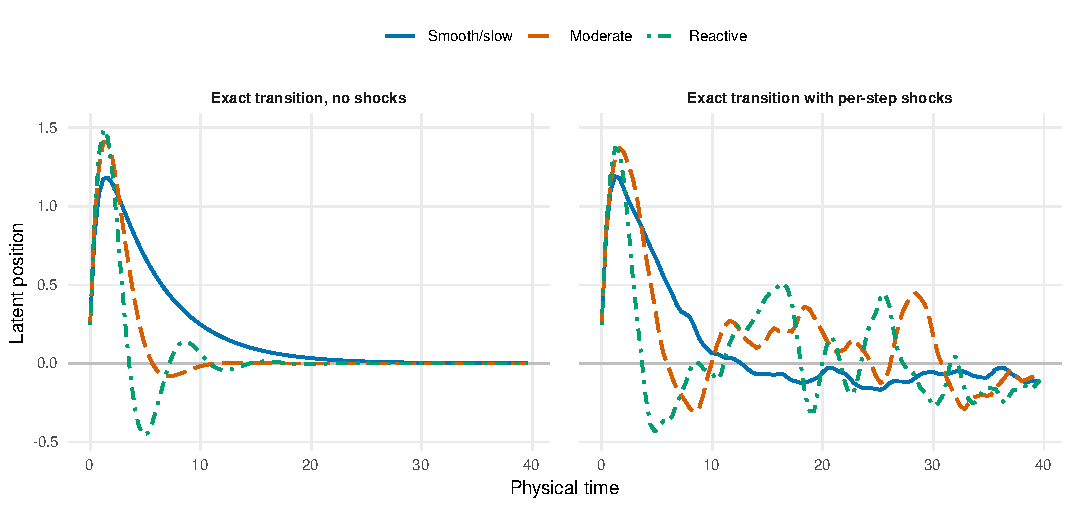
\includegraphics[width=0.9\linewidth,height=\textheight,keepaspectratio]{figures/lomm_three_factor_example.pdf}

}

\caption{\label{fig-latent-inputs}Illustrative latent trajectories for
three uncoupled dimensions under the exact transition, shown without and
with piecewise-constant acceleration inputs. The inputs create irregular
peaks and reversals while the feedback parameters govern the underlying
dynamic regime.}

\end{figure}%

\subsection{A.2 Dynamic Regimes and Finite-Horizon
Amplification}\label{a.2-dynamic-regimes-and-finite-horizon-amplification}

The characteristic roots describe whether the deterministic motion
decays, grows, or oscillates. For dimension \(f\), they are

\[
r_{f,\pm}=\frac{\zeta_f\pm\sqrt{\zeta_f^2+4\eta_f}}{2}.
\]

Asymptotic stability means that the effect of an initial state
eventually decays to zero in the absence of new inputs. In continuous
time, it requires \(\eta_f<0\) and \(\zeta_f<0\), and the roots are
oscillatory when \(\zeta_f^2+4\eta_f<0\). For the sampled transition,
the spectral radius \(\rho\) is the largest absolute eigenvalue of
\(\boldsymbol\Phi_f(\Delta)\). Stability requires

\[
\rho\{\boldsymbol{\Phi}_f(\Delta)\}
=\exp\!\left[\Delta\max\{\operatorname{Re}(r_{f,+}),\operatorname{Re}(r_{f,-})\}\right]<1.
\]

The real parts of the characteristic roots determine whether the effect
of an initial state decays or grows. Over the observation horizon
\(H=(T-1)\Delta\), we summarize this modal change by

\[
g_f(H)=\exp\!\left[H\max\{\operatorname{Re}(r_{f,+}),\operatorname{Re}(r_{f,-})\}\right].
\]

This quantity describes deterministic modal growth or decay. It does not
bound individual stochastic trajectories or capture all possible
transient amplification. Table C6 reports the maximum real part of the
roots and the modal factors, while Table C5 summarizes the amplitudes
actually produced by the generator. Activity modulation can create
additional nonstationarity and is reported separately. The amplifying
configurations are finite-record stress tests.

\subsection{A.3 Initial States}\label{a.3-initial-states}

The system is uncoupled: \(\eta_f\), \(\zeta_f\), and \(\sigma_{qf}\)
may vary by dimension, and a dimension does not directly change the
level or velocity of another dimension.

Study 1 initialized every dimension independently at the start of each
uninterrupted segment by drawing
\(\mathbf s_{if,1}=(x_{if,1},v_{if,1})^\top\) from its zero-mean
stationary Gaussian distribution. A new state was drawn after each
interruption.

Study 2's primary simulation design initialized every dimension in every
clip at \(x_{if,1}=0.25\) and \(v_{if,1}=2\). The sensitivity analysis
replaced these common fixed values with draws that were independent
across dimensions and clips.

For a stable dimension, the stationary covariance \(\mathbf P_f\) solves

\[
\mathbf{P}_f=\boldsymbol{\Phi}_f(\Delta)\mathbf{P}_f\boldsymbol{\Phi}_f(\Delta)^\top
+\boldsymbol{\Gamma}_f(\Delta)\sigma_{qf}^2\boldsymbol{\Gamma}_f(\Delta)^\top,
\]

whose solution is unique when \(\rho\{\boldsymbol{\Phi}_f(\Delta)\}<1\).
Drawing \(\mathbf{s}_{if,1}\sim\mathcal{N}(\mathbf{0},\mathbf{P}_f)\)
makes the state process stationary before the activity layer is applied;
time-varying activity modulation still renders \(a_{if}(t)x_{if}(t)\)
nonstationary.

For a dimension with positive velocity feedback, the sensitivity draws
\(x_{if,1}\sim\mathrm{Unif}(-0.25,0.25)\) and
\(v_{if,1}\sim\mathrm{Unif}(-2,2)\). The alternative therefore changes
cross-dimension and cross-clip coherence, marginal means, covariance,
stationarity, and the magnitude and direction of the initial transient;
the observed horizon is unchanged.

\subsection{A.4 The Activity Layer at a
Transition}\label{a.4-the-activity-layer-at-a-transition}

Changes in an observed indicator can arise from changes in the latent
level or changes in its activity multiplier. For the expressed signal
\(\tilde{x}_{if,n}=a_{if,n}x_{if,n}\),

\[
\frac{\tilde{x}_{if,n+1}-\tilde{x}_{if,n}}{\Delta}
=a_{if,n+1}\frac{x_{if,n+1}-x_{if,n}}{\Delta}
+\frac{a_{if,n+1}-a_{if,n}}{\Delta}x_{if,n}.
\]

The first term is latent change expressed at the new activity level. The
second is change caused by the activity multiplier. An abrupt activity
transition can therefore contribute strongly to an estimated derivative
even though the latent level remains continuous. The gradual-transition
sensitivity analysis examines whether recovery depends on these abrupt
changes. At each observation, activity multiplies the completed latent
state at the same observation index.

The activity schedule takes two nonnegative values,
\(a_{\mathrm{high}}\) and \(a_{\mathrm{low}}\). In non-switching
families the dominant dimension remains at \(a_{\mathrm{high}}\) for the
whole record and the others remain at \(a_{\mathrm{low}}\). In switching
families, dwell fractions determine how long each dimension remains
dominant before the schedule reassigns \(a_{\mathrm{high}}\). Appendix B
lists the numeric gains and dwell values used in the Study 2 families.

\subsection{A.5 The Observation Layer}\label{a.5-the-observation-layer}

LOMM has two observation models. The continuous-indicator model maps
latent processes directly to observed variables with specified loadings
and measurement error. The bounded-score model first generates log-ratio
coordinates and then converts them to positive scores that sum to one.
Its ILR coordinates combine the logarithms of multiple score channels;
there is no separate ILR coordinate for each channel. We use separate
notation for continuous indicators, \(\mathbf z\), and log-ratio
coordinates, \(\mathbf u\).

Let \(J\) denote the number of positive score channels, let \(d=J-1\),
and let \(\mathbf V\in\mathbb R^{J\times d}\) be a fixed orthonormal
isometric log-ratio (ILR) basis satisfying
\(\mathbf V^\top\mathbf V=\mathbf I_d\) and
\(\mathbf V^\top\mathbf 1_J=\mathbf 0\). The Study 1 basis used here is
a normalized Helmert basis constructed in the stated 11-channel order.
The full observation model in log-ratio coordinates is

\[
\mathbf u_{in}
=
\boldsymbol\mu^{(u)}+\mathbf b_i^{(u)}
+\kappa s_i^{(u)}
\left(
\boldsymbol\Lambda_i^{(u)}\tilde{\mathbf x}_{in}
+\boldsymbol\varepsilon_{in}^{(u)}
\right).
\]

Here
\(\mathbf u_{in},\boldsymbol\mu^{(u)},\mathbf b_i^{(u)},\boldsymbol\varepsilon_{in}^{(u)}\in\mathbb R^d\),
\(s_i^{(u)}>0\) is the clip scale, \(\kappa>0\) is a global scale, and
\(\boldsymbol\Lambda_i^{(u)}\in\mathbb R^{d\times m}\) maps the \(m\)
activity-scaled latent positions into the log-ratio coordinates. The
residual covariance is
\(\boldsymbol\Sigma_i^{(u)}\in\mathbb R^{d\times d}\), with
\(\boldsymbol\varepsilon_{in}^{(u)}\mid\boldsymbol\Sigma_i^{(u)}\sim\mathcal N(\mathbf 0,\boldsymbol\Sigma_i^{(u)})\).
The clip scale multiplies both signal and residual, and the baseline is
additive.

The continuous-indicator branch has output dimension \(p\) and uses
separate measurement parameters:

\[
\mathbf z_{in}
=
\mathbf b_i^{(z)}
+s_i^{(z)}
\left(
\boldsymbol\Lambda_i^{(z)}\tilde{\mathbf x}_{in}
+\boldsymbol\varepsilon_{in}^{(z)}
\right),
\qquad
\boldsymbol\varepsilon_{in}^{(z)}\mid\boldsymbol\Psi_i
\sim\mathcal N(\mathbf 0,\boldsymbol\Psi_i),
\]

where
\(\mathbf z_{in},\mathbf b_i^{(z)},\boldsymbol\varepsilon_{in}^{(z)}\in\mathbb R^p\),
\(\boldsymbol\Lambda_i^{(z)}\in\mathbb R^{p\times m}\),
\(\boldsymbol\Psi_i\in\mathbb R^{p\times p}\), and \(s_i^{(z)}>0\). In
both branches, residuals are conditionally independent over time and
across clips and are independent of latent states, initial states,
activity schedules, and acceleration inputs. Designs with fixed
measurement parameters use a common loading matrix and residual
covariance within the relevant branch.

The residual-correlation sensitivity condition applies to the continuous
indicators and sets

\[
\boldsymbol\Psi
=s_\varepsilon^2
\left\{(1-\rho)\mathbf I_p
+\rho\mathbf 1_p\mathbf 1_p^\top\right\},
\qquad \rho=0.10,
\]

which introduces residual covariance between every pair of the \(p\)
indicators, including pairs from different prespecified blocks.

The baseline constructions are also branch-specific. Study 1 draws
\(\mathbf b_i^{(u)}\) from a zero-mean Gaussian whose covariance is
estimated from MAFW calibration videos in the full \(d\)-dimensional
log-ratio coordinate space. Study 2's between-clip-variability analysis
uses

\[
\mathbf b_i^{(z)}
=\boldsymbol\Lambda^{(z)}\boldsymbol\beta_i,
\qquad E(\boldsymbol\beta_i)=\mathbf 0,
\]

so that between-clip variation stays within the column space of the
continuous-indicator loading matrix. Study 2 conditions without baseline
and scale differences set \(\mathbf b_i^{(z)}=\mathbf 0\) and
\(s_i^{(z)}=1\), giving

\[
\mathbf z_{in}
=\boldsymbol\Lambda_i^{(z)}\tilde{\mathbf x}_{in}
+\boldsymbol\varepsilon_{in}^{(z)}.
\]

This equation defines the continuous indicators used in Study 2's
primary recovery designs before any bounded-score mapping. Each of the
\(p=mk\) indicators loads on one dimension and has diagonal measurement
error. In the matched-method and extended factorial designs, each
primary loading receives an independent
\(\operatorname{Unif}(-0.15,0.15)\) deviation from its nominal value,
and each residual variance receives an independent
\(\operatorname{Unif}(-0.01,0.01)\) deviation from \(s_\varepsilon^2\).
The one-at-a-time sensitivity and between-clip-variability designs use
fixed equal values except where the stated condition changes them. Zero
baseline and unit scale remove baseline and overall-scale differences;
common loadings and residual covariance require the separate
fixed-parameter condition.

For bounded output, LOMM converts the coordinates to strictly positive
scores that sum to one, the open probability simplex. The centered
log-ratio (CLR) expresses each channel relative to the geometric mean of
all channels. The isometric log-ratio (ILR) represents the same
information in \(d=J-1\) orthonormal coordinates. Formally,

\[
\operatorname{clr}(\mathbf p)
=\log\mathbf p-
J^{-1}\{\mathbf 1_J^\top\log(\mathbf p)\}\mathbf 1_J,
\qquad
\operatorname{ilr}_{\mathbf V}(\mathbf p)
=\mathbf V^\top\operatorname{clr}(\mathbf p),
\]

with the logarithm applied componentwise. For the canonical bounded LOMM
output, applying softmax to \(\mathbf V\mathbf u_{in}/\tau\) gives

\[
\operatorname{ilr}_{\mathbf V}(\mathbf p_{in})=\frac{\mathbf u_{in}}{\tau},
\qquad
\operatorname{clr}(\mathbf p_{in})
=\frac{\mathbf V\mathbf u_{in}}{\tau},
\]

The second identity follows because the components of
\(\mathbf V\mathbf u_{in}\) sum to zero. The fixed basis excludes the
unidentified common-logit direction and the softmax produces strictly
positive rows summing to one, so the scores identify the scaled
coordinates \(\mathbf u_{in}/\tau\) exactly. A common-logit component
remains unobservable, and the unscaled coordinates and \(\tau\) are not
separately identified without an external scale constraint.

The Study 2 bounded-score sensitivity condition uses the \(p=mk\)
continuous-indicator vector directly. With \(J=p\), it computes

\[
\mathbf p^{\mathrm{dep}}_{in}
=\operatorname{softmax}\left(\frac{\mathbf z_{in}}{\tau}\right),
\qquad
\operatorname{clr}\!\left(\mathbf p^{\mathrm{dep}}_{in}\right)
=\frac{1}{\tau}\mathbf P_p\mathbf z_{in},
\qquad
\mathbf P_p
=\mathbf I_p-\frac{\mathbf 1_p\mathbf 1_p^\top}{p}.
\]

For any orthonormal ILR basis
\(\mathbf V_p\in\mathbb R^{p\times(p-1)}\),
\(\mathbf V_p\mathbf V_p^\top=\mathbf P_p\). Defining
\(\mathbf u^{\mathrm{dep}}_{in}=\mathbf V_p^\top\mathbf z_{in}\)
therefore gives
\(\mathbf V_p\mathbf u^{\mathrm{dep}}_{in}=\mathbf P_p\mathbf z_{in}\).
Softmax is invariant to the removed row mean, so the direct-softmax
branch is equivalent to applying the basis form to
\(\mathbf u^{\mathrm{dep}}_{in}\). The analysis used the \(p\) raw
scores and the \(p\) CLR components, which satisfy a zero-sum
constraint; it did not analyze the \((p-1)\) ILR coordinates. The
common-logit direction in \(\mathbf z_{in}\) is unidentifiable after
this transformation.

In the equal-loading reference condition used for this sensitivity, an
equal increase in all expressed latent levels adds the same amount to
every logit. Softmax removes this common component. Specifically,
\(\boldsymbol\Lambda^{(z)}\mathbf 1_m=\lambda\mathbf 1_p\), so
\(\mathbf P_p\boldsymbol\Lambda^{(z)}\mathbf 1_m=\mathbf 0\). The
projected loading matrix \(\mathbf P_p\boldsymbol\Lambda^{(z)}\) has
rank \(m-1\), leaving one fewer independent latent direction. The
transformation therefore changes the latent representation as well as
the associations among indicators. The original channel grouping may
still contain recoverable information; this sensitivity analysis tests
whether methods recover that grouping after the transformation.

\subsection{A.6 Converting Period and Damping to Feedback
Parameters}\label{a.6-converting-period-and-damping-to-feedback-parameters}

The Study 1 calibration search specified dynamics by natural period and
damping ratio. The following equations convert those settings to the
feedback parameters \(\eta_f\) and \(\zeta_f\). If \(P_f\) is the
natural period in observation intervals and \(\xi_f\) is the damping
ratio, then

\[
\omega_{n,f}=\frac{2\pi}{P_f\Delta},
\qquad
\eta_f=-\omega_{n,f}^2,
\qquad
\zeta_f=-2\xi_f\omega_{n,f},
\]

and the damped angular frequency is
\(\omega_{d,f}=\omega_{n,f}\sqrt{1-\xi_f^2}\). With the Study 1 settings
\(P_f=12\), \(\xi_f=0.20\), and \(\Delta=1\), these give
\(\eta_f=-0.2742\) and \(\zeta_f=-0.2094\). The acceleration inputs were
scaled to give unit stationary position variance.

\subsection{A.7 Identifiability}\label{a.7-identifiability}

The simulations fix the generating parameters in advance. Estimating
them from observed data would require additional constraints because
different parameter combinations can produce the same observations. The
main ambiguities concern scale, dimension labels, and sampling
frequency.

For either observation branch \(h\in\{u,z\}\) and any nonsingular
diagonal matrix \(\mathbf{D}\),

\[
\boldsymbol{\Lambda}^{(h)}\tilde{\mathbf{x}}_{in}
=(\boldsymbol{\Lambda}^{(h)}\mathbf{D}^{-1})(\mathbf{D}\tilde{\mathbf{x}}_{in}),
\]

so loading magnitude and latent-trajectory scale are not jointly
identified without an explicit scale constraint. Activity gain and
acceleration-input scale contribute to latent amplitude in the same way.
The softmax layer adds invariance to a common location shift and a
tradeoff between the temperature and the coordinate scale. Dimension
labels are recoverable only up to permutation.

Sampling creates another ambiguity: different oscillation frequencies
can produce the same values at the observation times. This is called
aliasing. For an underdamped dimension, write

\[
r_{f,\pm}=\frac{\zeta_f}{2}\pm i\omega_f,
\qquad
\omega_f=
\frac{1}{2}\sqrt{-(\zeta_f^2+4\eta_f)}.
\]

At observation times \(t_n=(n-1)\Delta\), the frequencies \(\omega_f\)
and \(\omega_f+2\pi q/\Delta\) for integer \(q\) generate the same
sampled sine and cosine sequences after an appropriate change in initial
velocity. Identifying continuous-time oscillator parameters from data
therefore requires a cadence-dependent restriction such as

\[
0<\omega_f<\frac{\pi}{\Delta},
\]

together with a specified acceleration-input model and constraints on
the latent state basis. Together, these ambiguities require sign and
scale constraints on the dimensions, normalization of the activity
schedule, anchoring of either the loading scale or the input scale, a
reference-logit or sum-to-zero constraint, a fixed or otherwise
identified temperature, and this frequency restriction.

Every oscillatory mode used here satisfies the frequency restriction. In
Study 1, the selected damped angular frequency is approximately 0.513
radians per observation; the largest frequency in the calibration search
is approximately 0.524. Both are below the sampling bound of \(\pi\).
Study 2 uses \(\Delta\in\{0.25,0.4\}\), giving bounds of approximately
12.57 and 7.85 against a largest angular frequency of approximately
1.04. The simulations do not estimate any of these parameters.

\newpage

\setcounter{table}{0}
\renewcommand{\thetable}{B\arabic{table}}
\setcounter{figure}{0}
\renewcommand{\thefigure}{B\arabic{figure}}

\section{Appendix B: Study Designs and Implementation
Details}\label{appendix-b-study-designs-and-implementation-details}

This appendix gives the design and implementation details for both
studies. Study 1 evaluates resemblance to real bounded-score series.
Study 2 evaluates recovery of a prespecified factor structure from
continuous indicators.

\subsection{B.1 Study 1 Scoring and
Calibration}\label{b.1-study-1-scoring-and-calibration}

The sample contains 100 MAFW videos selected across the available
expression categories. Category labels served only to stratify sampling
and fold construction. The analysis retained 3,557 complete observations
in 188 uninterrupted segments. Individual videos contain 16 to 50
complete observations, with a median of 35. Segment lengths range from 1
to 50 observations, with a median of 13.5.

transforEmotion sampled up to 50 frames uniformly from each video and
used OpenAI CLIP ViT-Large/14. A Haar cascade detected faces, and the
largest detected face was expanded by 50 pixels on each side before
classification. Frames without a detected face received missing scores.
Eleven lowercase labels were passed directly to the text encoder: anger,
disgust, fear, happiness, neutral, sadness, surprise, contempt, anxiety,
helplessness, and disappointment. Burned-in subtitles were not masked
when they fell inside the padded face crop.

Scores were required to lie in \([0,1]\). A complete row was retained
when its sum was positive, finite, and within \(10^{-6}\) of one, then
divided by that sum in the fixed channel order. Values were not
truncated, and zero replacement was disabled. The transformation stops
with an error if a complete row contains a zero. None of the 39,127
retained scores equaled zero; the minimum before row normalization was
approximately \(2.42\times10^{-5}\). The analysis used complete
observations and preserved the uninterrupted segment boundaries.

\emph{Features and segment boundaries.} The evaluation panel contains
eleven statistics: median level, interquartile range of levels,
interquartile range of changes, lag-1 autocorrelation, run-length
entropy, sample entropy, permutation entropy, spectral entropy,
effective rank, robust level variance, and robust change variance. The
eight univariate statistics were computed for each of the eleven score
channels and each of their eleven CLR coordinates. The three joint
statistics used the score panel and its ten ILR coordinates. For each
video, the median of the finite channel values summarized each
univariate statistic. Together with the joint statistics, these
summaries give 22 features. A feature remained undefined if no channel
had a finite value.

Levels were pooled across all retained observations within a video.
Changes and lagged pairs were formed within segments and then pooled
across the video; no pair crossed a segment boundary. Lag-1 correlation
was computed from these pooled pairs. Run lengths were formed separately
within segments, after removing zero changes, capped at eight, and
pooled across segments. Sample and permutation entropy pooled windows
formed entirely within segments. Sample entropy compared these valid
windows across the video, including windows from different segments.
Spectral entropy was computed separately for each eligible segment and
averaged using segment length minus one as the weight. A segment
containing one observation contributed to level statistics but supplied
no changes, lagged pairs, or entropy windows.

Change IQR and robust change variance required at least one
within-segment change. Lag-1 correlation required at least two pairs and
nonzero variation in the first and second observations in the pairs.
Run-length entropy required four observations across the video and was
zero when fewer than two runs remained.

Sample entropy used order 2, windows of three observations, and a
tolerance of 0.20 times the channel's standard deviation across the
video. It required at least two windows and used the negative logarithm
of \((A+0.5)/(B+1)\), where \(A\) counts matching pairs of
three-observation windows and \(B\) counts matches between their first
two observations; a zero or undefined channel standard deviation
produced zero. Permutation entropy used order 3, required at least two
windows, and resolved ties by position within the window.

Spectral entropy required segments of at least eight observations with
positive total spectral power and at least two positive frequency
powers. Statistics failing their requirements remained undefined.

Effective rank used the positive eigenvalues of the video correlation
matrix and required that matrix to be finite. Robust level variance was
the 10\% trimmed mean squared distance from the video center divided by
the coordinate dimension. Robust change variance was the 10\% trimmed
mean squared within-segment first difference divided by twice the
coordinate dimension. The joint statistics required at least two
observations.

\emph{Calibration.} The 100 videos were divided into four
category-stratified folds. Each fold used 75 calibration videos and 25
evaluation videos. The calibration videos determined the coordinate
center, loading subspace, between-video baseline covariance, and
empirical distribution of within-video scale. The first three
eigenvectors of the pooled within-video covariance supplied the loading
directions. The between-video baseline covariance was shrunk halfway
toward its diagonal, and its eigenvalues were floored at \(10^{-8}\).
The generator included between-video baseline and scale variation.
Activity modulation was disabled: every latent dimension had an activity
multiplier of one at every generated observation.

Generator settings were selected within each calibration set. The
dynamic search crossed periods of 12, 24, and 48 observations with
damping ratios of 0.01, 0.05, and 0.20. Selection used the interquartile
range of changes, lag-1 autocorrelation, run-length entropy, and
spectral entropy. Conditional on the selected dynamics, the measurement
search crossed residual standard deviations of 0.10, 0.20, and 0.30 with
\(\kappa\) values of 0.75, 1.00, and 1.25. Measurement selection used 16
discrepancy components: median level, level IQR, change IQR, lag-1
autocorrelation, run-length entropy, spectral entropy, effective rank,
and total variance, each for scores and log-ratios. Total variance was
the sum of the coordinate variances. The additional entropy and robust
variance statistics belonged to the subsequent 22-feature evaluation.
Each candidate was evaluated with three calibration simulations. All
four folds selected a period of 12 observations, damping ratio 0.20,
residual standard deviation 0.30, and \(\kappa=0.75\).

The static logistic-normal generator used the same calibrated coordinate
center, covariance geometry, between-video baseline and scale
distributions, observation positions, and segment boundaries. It drew
independent log-ratio observations within each video. Each selected
generator produced 100 datasets per fold with 25 simulated series in
each dataset.

\emph{Evaluation.} The MAFW reference used 1,000 comparisons per fold.
Each comparison drew two disjoint, category-stratified groups of 25
videos from the 75 calibration videos. Every feature was standardized by
the median and scale of its finite values in the calibration videos. The
scale was the IQR, with successive fallbacks to 1.4826 times the median
absolute deviation, the standard deviation, and one; a data-derived
scale had to exceed \(10^{-8}\). Before standardization, any undefined
video feature was replaced by its calibration median and therefore
became zero after standardization. This replacement used no evaluation
videos. One MAFW video had no segment of eight observations, leaving its
two spectral-entropy features undefined; these were the only two
undefined values among the 2,200 empirical video features. The distance
between two series was the root-mean-square Euclidean distance across
all 22 standardized features, including features replaced in this way.
The fold-specific similarity threshold was the 95th percentile of the
pooled directional nearest-neighbor distances between the two MAFW
groups.

For each generated dataset, plausibility was the proportion of its 25
simulated series whose nearest MAFW evaluation series fell within the
threshold. Coverage was the proportion of the 25 MAFW evaluation series
whose nearest simulated series fell within the threshold. Results were
averaged across the four folds. The reported ranges are the 2.5th and
97.5th percentiles across the 100 generated datasets or 1,000 MAFW
reference comparisons.

\emph{Distributional comparisons.} Calibration and metric-specific
distributional discrepancy used finite channel-by-video contributions
for each univariate statistic, and one contribution per video for each
joint statistic. For univariate statistics, these distributions pooled
channel values across videos. Undefined contributions were omitted
separately from the empirical and simulated distributions. Their
absolute median difference and one-dimensional Wasserstein distance were
divided by the calibration scale, using the same scale fallback rule,
and the larger standardized value was retained. The measurement
objective averaged its 16 components, giving equal weight to scores and
log-ratios; an entirely undefined component made the full selection loss
infinite. All stored calibration objectives were finite. The reported
full distributional discrepancy averaged the 22 evaluation components.

\subsection{B.2 Study 2 Simulation
Designs}\label{b.2-study-2-simulation-designs}

For each clip, LOMM sets or draws the starting state and acceleration
inputs according to the configuration, advances each latent dimension,
applies the activity schedule, and constructs the observed indicators.
The primary, shorter-series, and extended factorial designs use
continuous indicators. All clips share the same indicator assignments
and nominal measurement parameters. The generator draws clip-specific
loading and residual-variance perturbations as specified in the
random-draw table below. The one-at-a-time sensitivity conditions use
fixed equal measurement parameters except for the stated change.

\begin{table}[H]

\caption{\label{tbl-scenario-families}The six Study 2 scenario families.
Dwell values are fractions of the number of observations per clip.}

\centering{

\begingroup\scriptsize\setlength{\tabcolsep}{3pt}

\begin{tabular}{cp{1.75in}cccp{1.25in}}
\toprule
Code & Family & Switching & Active / background gain & Dwell fraction & Dynamic rule\\
\midrule
A & Weak expression, one dominant dimension & No & 0.35 / 0.05 & 1.00 / 1.00 & Stable, low input scale\\
B & Strong expression, one dominant dimension & No & 1.00 / 0.08 & 1.00 / 1.00 & Stable, standard input scale\\
C & Strong expression, switching dominant dimension & Yes & 1.00 / 0.08 & 0.20 / 0.45 & Stable, standard input scale\\
D & Strong expression, rapid switching & Yes & 1.25 / 0.08 & 0.03 / 0.10 & Stable, high input scale\\
E & Amplifying dynamics, one dominant dimension & No & 1.00 / 0.08 & 1.00 / 1.00 & Positive velocity feedback\\
\addlinespace
F & Amplifying dynamics, switching dominant dimension & Yes & 1.10 / 0.10 & 0.12 / 0.30 & Positive velocity feedback\\
\bottomrule
\end{tabular}
\endgroup

}

\end{table}%

In non-switching scenarios, one dimension remains dominant for a whole
clip and the dominant dimension rotates across clips. Switching
scenarios sample dwell intervals and change the dominant dimension over
time. Families A through D use stable dynamics. Families E and F use
positive velocity feedback and test recovery under finite-horizon
amplification.

The dynamic parameters are listed in Table B2. Each vector gives one
value per latent dimension. The primary and shorter designs use
\(\Delta=0.4\); the extended design with 300 observations uses
\(\Delta=0.25\). The displayed \(\sigma_q\) values are input standard
deviations per transition. Holding them fixed while changing \(\Delta\)
changes the input specification per unit of time.

\begingroup\scriptsize\setlength{\tabcolsep}{4pt}
\begin{table}[H]

\caption{Dynamic parameters for each scenario family. Entries in each vector follow the dimension order. Acceleration-input SD is the per-step standard deviation $\sigma_q$. Four-dimensional conditions occur only in the extended factorial simulation.}
\centering
\footnotesize
\setstretch{1}

\begin{tabular}[t]{ccp{1.70in}p{1.70in}p{1.65in}}
\toprule
Code & $m$ & $\eta$ & $\zeta$ & Acceleration-input SD\\
\midrule
A & 2D & -0.30; -0.55 & -1.70; -1.00 & 0.06; 0.15\\
A & 3D & -0.30; -0.55; -0.85 & -1.70; -1.00; -0.65 & 0.06; 0.15; 0.23\\
A & 4D & -0.30; -0.55; -0.85; -1.10 & -1.70; -1.00; -0.65; -0.30 & 0.06; 0.15; 0.23; 0.33\\
B & 2D & -0.30; -0.55 & -1.70; -1.00 & 0.12; 0.30\\
B & 3D & -0.30; -0.55; -0.85 & -1.70; -1.00; -0.65 & 0.12; 0.30; 0.45\\
\addlinespace
B & 4D & -0.30; -0.55; -0.85; -1.10 & -1.70; -1.00; -0.65; -0.30 & 0.12; 0.30; 0.45; 0.65\\
C & 2D & -0.30; -0.55 & -1.70; -1.00 & 0.12; 0.30\\
C & 3D & -0.30; -0.55; -0.85 & -1.70; -1.00; -0.65 & 0.12; 0.30; 0.45\\
C & 4D & -0.30; -0.55; -0.85; -1.10 & -1.70; -1.00; -0.65; -0.30 & 0.12; 0.30; 0.45; 0.65\\
D & 2D & -0.30; -0.55 & -1.70; -1.00 & 0.15; 0.38\\
\addlinespace
D & 3D & -0.30; -0.55; -0.85 & -1.70; -1.00; -0.65 & 0.15; 0.38; 0.56\\
D & 4D & -0.30; -0.55; -0.85; -1.10 & -1.70; -1.00; -0.65; -0.30 & 0.15; 0.38; 0.56; 0.81\\
E & 2D & -0.05; -0.10 & 0.08; 0.10 & 0.25; 0.25\\
E & 3D & -0.05; -0.10; -0.15 & 0.08; 0.10; 0.12 & 0.25; 0.25; 0.25\\
E & 4D & -0.05; -0.10; -0.15; -0.20 & 0.08; 0.10; 0.12; 0.14 & 0.25; 0.25; 0.25; 0.25\\
\addlinespace
F & 2D & -0.05; -0.10 & 0.08; 0.10 & 0.35; 0.35\\
F & 3D & -0.05; -0.10; -0.15 & 0.08; 0.10; 0.12 & 0.35; 0.35; 0.35\\
F & 4D & -0.05; -0.10; -0.15; -0.20 & 0.08; 0.10; 0.12; 0.14 & 0.35; 0.35; 0.35; 0.35\\
\bottomrule
\end{tabular}
\end{table}\endgroup

The primary \(T=100\) design contains 21,600 datasets: 216 factorial
conditions with 100 paired replications per condition. The factorial
crosses six scenario families, \(m\in\{2,3\}\) dimensions,
\(N\in\{50,100\}\) clips, loadings \(\{0.40,0.60,0.80\}\), residual
standard deviations \(\{0.125,0.25,0.50\}\), and four indicators per
dimension. The shorter-series design generates 21,600 corresponding
datasets with \(T=25\), \(\Delta=0.4\), and duration 9.6. Every method
receives the same dataset within each condition and replication.

The one-at-a-time sensitivity analyses fix \(N=100\), \(T=100\), loading
0.60, residual standard deviation 0.25, and four indicators per
dimension (the reference condition). They cross all six families, two
dimensionalities, and 50 paired replications while changing one feature
at a time.

\begin{table}[H]

\caption{\label{tbl-challenge-variants}One-at-a-time sensitivity
conditions. Each changes one design component of the reference
condition.}

\centering{

\begingroup\scriptsize\setlength{\tabcolsep}{3pt}

\begin{tabular}{p{1.55in}p{4.75in}}
\toprule
Sensitivity condition & Specification\\
\midrule
Alternative initialization & Stationary zero-mean starts for stable dimensions; bounded independent starts for amplifying dimensions\\
Gradual activity transitions & A five-observation transition replaces each abrupt switch\\
Cross-loadings & Normal cross-loadings with pre-truncation SD 0.05, truncated to [-0.10, 0.10]\\
Residual equicorrelation & Correlation 0.10 between every residual pair, including pairs from different dimensions\\
Correlated inputs & Acceleration-input correlation 0.15 between dimensions\\
\addlinespace
Bounded scores & Direct softmax of the p indicators with tau = 1, analyzed as raw scores or CLR components\\
\bottomrule
\end{tabular}
\endgroup

}

\end{table}%

\begin{table}[H]

\caption{\label{tbl-random-draws}Random draws and perturbations.}

\centering{

\begingroup\scriptsize\setlength{\tabcolsep}{3pt}

\begin{tabular}{p{1.10in}p{1.25in}p{3.95in}}
\toprule
Component & Scope & Specification\\
\midrule
Acceleration input & Studies 1 and 2 & $\mathbf q_{i,n}\sim\mathcal N_m(\mathbf 0,\mathbf D_q\mathbf R_q\mathbf D_q)$. The primary designs use $\mathbf R_q=\mathbf I_m$; the correlated-input sensitivity sets every off-diagonal correlation to 0.15. Draws are independent across clips and transitions. Study 1 scales $\sigma_{qf}$ to give unit stationary position variance; Table B2 gives the Study 2 values.\\
Initial state & Study 1 & At the start of each uninterrupted segment, each dimension is drawn independently as $\mathbf s_{if,1}\sim\mathcal N_2(\mathbf 0,\mathbf P_f)$, where $\mathbf P_f$ is the stationary covariance for the selected transition and input scale.\\
Activity & Study 1 & Activity modulation is disabled: $a_{if,n}=1$ for every dimension and generated observation.\\
Primary loadings & Study 2 matched and extended designs & For item $j$ assigned to dimension $f$, $\Lambda_{i,jf}^{(z)}=\lambda+U_{ij}$ with independent $U_{ij}\sim\operatorname{Unif}(-0.15,0.15)$. All cross-loadings are zero.\\
Residual variances & Study 2 matched and extended designs & For indicator $j$, $\Psi_{i,jj}=s_\varepsilon^2+V_{ij}$ with independent $V_{ij}\sim\operatorname{Unif}(-0.01,0.01)$; off-diagonal entries are zero.\\
\addlinespace
Switching dwell & Study 2 switching families & Set $L_{\min}=\max\{1,\lfloor Td_{\min}\rfloor\}$ and $L_{\max}=\max\{L_{\min},\lceil Td_{\max}\rceil\}$. Each dwell is sampled uniformly from the integers $L_{\min},\ldots,L_{\max}$; the final dwell is truncated at observation $T$. The first dominant dimension rotates across clips, and each later dominant dimension is sampled uniformly from the other $m-1$ dimensions.\\
Cross-loadings & Study 2 sensitivity & Each non-primary loading is drawn independently from $\mathcal N(0,0.05^2)$ and truncated componentwise to $[-0.10,0.10]$. Primary loadings remain fixed at 0.60.\\
Factor baseline $\boldsymbol\beta_i$ & Study 2 between-clip analysis & $\boldsymbol\beta_i\sim\mathcal N_m(\mathbf 0,1.8487025519^2\mathbf I_m)$ and $\mathbf b_i^{(z)}=\boldsymbol\Lambda^{(z)}\boldsymbol\beta_i$.\\
Clip scale $s_i^{(z)}$ & Study 2 between-clip analysis & $s_i^{(z)}\sim\operatorname{Unif}(0.5,1.5)$, independently across clips. It multiplies the within-clip signal and measurement residual before the baseline is added.\\
\bottomrule
\end{tabular}
\endgroup

}

\end{table}%

The between-clip analysis uses 80 paired datasets from stable families A
through D, \(m\in\{2,3\}\), and 10 replications. Each dataset has
\(N=100\), \(T=100\), four indicators per dimension, loading 0.60,
residual standard deviation 0.25, and independent stationary starts. Its
baseline varies within the loading space according to
\(\boldsymbol\beta_i\sim\mathcal N_m(\mathbf 0,1.8487025519^2\mathbf I_m)\),
and its clip scale follows
\(s_i^{(z)}\sim\operatorname{Unif}(0.5,1.5)\).

The extended factorial simulation evaluates DynEGA on 518,400 datasets.
It crosses \(N\in\{50,100\}\), \(T\in\{100,300\}\), \(m\in\{2,3,4\}\),
\(k\in\{4,6\}\), three loading levels, three residual-error levels, six
scenarios, and 400 replications. The \(T=100\) conditions use
\(\Delta=0.4\) and the \(T=300\) conditions use \(\Delta=0.25\) while
holding per-step input variance fixed. Their difference therefore
combines the number of observations, the observation interval, the
physical duration, and the discrete input specification.

The public lomm\_observe() function implements the observation step and
records the configuration, seeds, and hashes needed for reproduction.
Study 2 uses the benchmark generator documented in the analysis code,
which returns continuous indicators for the primary designs and applies
the direct-softmax and CLR transformation for the bounded-score
sensitivity condition.

\subsection{B.3 Method
Implementations}\label{b.3-method-implementations}

DynEGA estimates first derivatives from time-delay embeddings,
constructs an EBICglasso partial-correlation network, and groups its
positive edges (\citeproc{ref-glla2010}{Boker et al., 2010};
\citeproc{ref-golino2019investigating}{H. Golino et al., 2020};
\citeproc{ref-golino2020modeling}{H. Golino et al., 2022};
\citeproc{ref-golino2017ega1}{H. F. Golino \& Epskamp, 2017}). Video
identity prevents embedding windows from crossing clip boundaries. An
explicit search selects the embedding dimension by the Total Entropy Fit
Index, with shorter embeddings breaking ties. Candidate dimensions are
\(\{5,10,15,25,50\}\) for \(T=100\) and \(\{5,6,10,12\}\) for \(T=25\).
EGAnet 2.3.0 uses GLLA embedding parameters tau = 1 and delta = 1, first
derivatives, automatic correlations, pairwise missing-data handling, and
the glasso model. The derivative scale does not affect the correlation
matrix because conversion from observation units to physical time
multiplies every derivative by the same positive constant.

Static EGA applies EBICglasso to the contemporaneous correlation matrix
of the stacked indicator levels and then uses the same
network-processing and community-detection rules as DynEGA. It ignores
the observation order. This makes it a benchmark that shows how much of
the grouping is recoverable without temporal information, and a
computational benchmark for the temporal procedures.

GraphicalVAR uses mlGraphicalVAR with clip identity as the grouping
variable, within-clip centering, variable standardization, and gamma 0.5
(\citeproc{ref-epskampggm}{Epskamp et al., 2018};
\citeproc{ref-graphicalVAR2024}{Epskamp, 2024}). Lagged pairs never
cross clip boundaries. The grouping uses the returned fixedPCC
contemporaneous residual partial-correlation matrix. The diagonal is
removed and the matrix is treated as an undirected weighted graph.

GIMME fits each standardized clip separately with unified structural
equation modeling and vector autoregression
(\citeproc{ref-gates2012group}{Gates \& Molenaar, 2012};
\citeproc{ref-lane2019uncovering}{Lane et al., 2019}). Standardized
residual covariance matrices from successful fits are aligned by
variable name, averaged across clips, and symmetrized. The resulting
graph is a residual-covariance graph. Unequal residual variances can
therefore influence its weights. This conversion was built for the
present comparison and differs from typical idiographic use.

For every method, negative graph weights are set to zero. If no positive
edge remains, absolute values of the original off-diagonal weights are
used; only an all-zero matrix produces singleton communities. The
integrated outputs do not record the frequency of this fallback. Louvain
at resolution 1.0 is primary (\citeproc{ref-blondel2008fast}{Blondel et
al., 2008}). Leiden and Walktrap are applied to the same fitted network
as sensitivity analyses (\citeproc{ref-pons2006walktrap}{Pons \& Latapy,
2005}; \citeproc{ref-traag2019leiden}{Traag et al., 2019}). A
deterministic offset from the dataset seed initializes each method fit.

GraphicalVAR and GIMME were omitted from the 518,400-dataset extended
factorial simulation because the full design was computationally
impractical. Both were included in the primary and shorter-series
designs. GraphicalVAR was also included in the one-at-a-time sensitivity
and between-clip analyses. GIMME was included in the between-clip
analysis and excluded from the one-at-a-time sensitivity analyses.

\subsection{B.4 Outcomes, Uncertainty, and
Computing}\label{b.4-outcomes-uncertainty-and-computing}

A method can fail to recover the generating dimensions because it
returns no usable network or because its network yields the wrong number
of groups. The primary recovery rate counts both outcomes as failures
and uses all attempted datasets as its denominator. We also report the
proportion of attempts that return a valid network and the proportion of
valid outputs with the correct number of dimensions. These supporting
rates separate computational failure from incorrect grouping.

Adjusted Rand index and variation of information compare the full
estimated and prespecified partitions among valid outputs. Higher
adjusted Rand index and lower variation of information indicate closer
agreement. Assignment accuracy matches estimated groups to dimensions to
maximize correct indicator assignments. Every indicator remains in the
denominator, and indicators in unmatched groups count as incorrect.

Trajectory diagnostics assess whether the recovered groups summarize the
time course of the generating processes. They are constructed from the
levels of the analyzed indicators after grouping, including for DynEGA.
Scores retain the original observation order within each clip. The
indicators are standardized over the pooled clips, and each recovered
group is summarized by its first principal component. A single-indicator
group uses its standardized indicator, and a row mean is used if a
component cannot be computed. Each resulting summary is then
standardized over the pooled clips. Let \(\mathbf y_{ig}\) denote the
summary of recovered group \(g\) in clip \(i\), and let
\(\tilde{\mathbf x}_{if}\) denote the activity-scaled trajectory of
data-generating dimension \(f\). The best-match absolute trajectory
correlation is

\[
R_{\mathrm{best}}
=
\frac{1}{Nm}
\sum_{i=1}^{N}\sum_{f=1}^{m}
\max_g
\left|
\operatorname{cor}
\left(\tilde{\mathbf x}_{if},\mathbf y_{ig}\right)
\right|.
\]

Correlations use pairwise complete observations. The maximizing
recovered group is selected separately for each data-generating
dimension, so the same recovered-group summary may be selected for
multiple dimensions.

Normalized root mean squared error (NRMSE) measures the difference
between the standardized trajectories. It uses a separate one-to-one
assignment within each clip. For data-generating dimension \(f\) and
recovered group \(g\), the sign-invariant cost is

\[
d_{ifg}
=
\min_{\delta\in\{-1,1\}}
\left[
\frac{1}{K_{ifg}}
\sum_{n\in\mathcal O_{ifg}}
\left\{
\frac{\tilde{x}_{if,n}-\bar{x}_{if}}{s_{x,if}}
-\delta
\frac{y_{ig,n}-\bar{y}_{ig}}{s_{y,ig}}
\right\}^{2}
\right]^{1/2},
\]

where \(\mathcal O_{ifg}\) contains the \(K_{ifg}\) observations for
which both standardized series are finite. The means and sample standard
deviations are computed separately for each series within each clip. Let
\(\mathcal O_{x,if}\) contain the \(K_{x,if}\) finite observations of
the activity-scaled latent trajectory. Its sample variance is

\[
s_{x,if}^{2}
=
\frac{1}{K_{x,if}-1}
\sum_{n\in\mathcal O_{x,if}}
\left(\tilde{x}_{if,n}-\bar{x}_{if}\right)^2,
\]

and \(s_{y,ig}^{2}\) is defined analogously for the recovered-group
summary. Thus, NRMSE is the root mean squared difference between two
within-clip standardized series after choosing the sign that gives the
smaller value.

For each clip, a linear assignment algorithm selects the one-to-one
matching \(\widehat\pi_i\) that minimizes the total cost. A comparison
with fewer than three finite pairs after standardization, including
comparisons involving a constant series, receives a cost of 2. The cost
matrix is padded with a value of 2 when a data-generating dimension has
no recovered-group match. The dataset-level diagnostic is

\[
\operatorname{NRMSE}
=
\frac{1}{Nm}
\sum_{i=1}^{N}\sum_{f=1}^{m}
d_{if,\widehat\pi_i(f)}.
\]

Correlation allows several latent dimensions to share the same recovered
summary; NRMSE assigns a different summary to each matched dimension.
All-attempt failure-adjusted versions assign correlation 0 and NRMSE 2
when no valid network output exists or the corresponding dataset
diagnostic is undefined.

Uncertainty uses 2,000 bootstrap resamples of whole datasets within each
reported analysis group. Monte Carlo standard errors use
delete-one-dataset jackknifing. The three community-detection algorithms
reuse the same fitted structure and therefore assess the grouping step
rather than estimator variability.

Analyses used R 4.5.1 on Rocky Linux 8.8 with dual Intel Xeon Silver
4310 processors, 48 logical threads, and 125 GiB RAM. Key versions were
EGAnet 2.3.0, graphicalVAR 0.3.4, gimme 10.0, igraph 2.2.1, qgraph
1.9.8, psych 2.5.6, lavaan 0.6-20, dplyr 1.1.4, and ggplot2 4.0.1.
GraphicalVAR and GIMME used a 900-second limit per fit in the primary
and shorter designs.

Runtime is elapsed wall-clock time for attempts returning a valid
network output. It includes structure estimation, network extraction,
and community detection. One fitted structure is reused for Louvain,
Leiden, and Walktrap, so feasibility counts unique fits and accuracy
counts fit-and-algorithm results. Runtime values are specific to this
implementation and machine.

\section{Appendix C: Supplementary
Results}\label{appendix-c-supplementary-results}

\setcounter{table}{0}
\renewcommand{\thetable}{C\arabic{table}}
\setcounter{figure}{0}
\renewcommand{\thefigure}{C\arabic{figure}}

\subsection{C.1 Metric-Level Results for Study
1}\label{c.1-metric-level-results-for-study-1}

Figure~\ref{fig-mafw-metric-benchmark} compares LOMM with the
MAFW-to-MAFW reference for each of the 22 features. Fourteen LOMM
discrepancies fell within the reference range. The full 22-feature
distributional discrepancy was 0.2543 {[}0.2356, 0.2738{]} for LOMM and
0.1811 {[}0.1521, 0.2193{]} for the MAFW reference. The corresponding
median for the static logistic-normal generator was 0.6942.

LOMM closely reproduced most measures of level, dispersion, short-term
change, persistence, effective dimensionality, and robust variation. Its
largest departures occurred for entropy. Sample entropy was higher and
spectral entropy was lower than in MAFW for both scores and log-ratio
coordinates. Log-ratio permutation entropy was lower, effective rank was
higher, and robust level variance was lower. The score median-level
discrepancy was just outside the reference range, although the signed
median difference was 0.004.

Diagnostic subsets gave the same interpretation. A time-domain subset
containing level, spread, change, lag-1 autocorrelation, and run-length
entropy had a LOMM discrepancy of 0.1463, within the MAFW reference
interval {[}0.0967, 0.1489{]}. A local-temporal subset containing
change, lag-1 autocorrelation, and run-length entropy also fell within
its reference interval. The two robust variance measures together fell
within the MAFW reference range. The entropy measures accounted for most
of the remaining full-panel discrepancy.

\begin{figure}[H]

\centering{

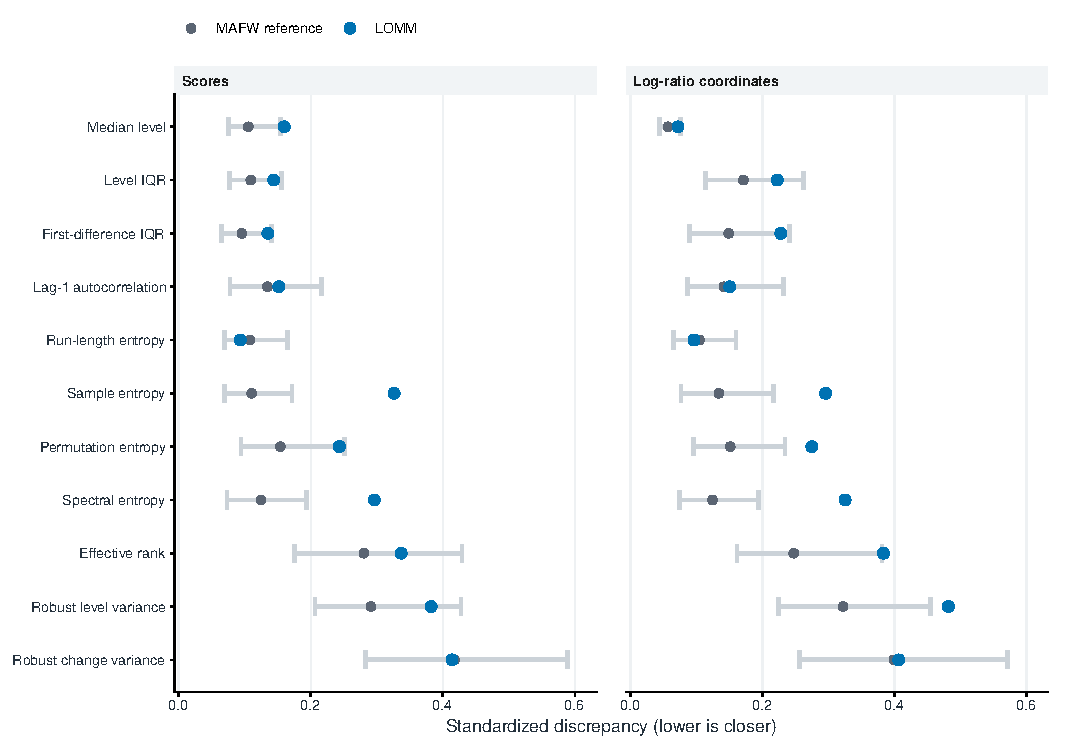
\includegraphics[width=0.95\linewidth,height=\textheight,keepaspectratio]{figures/figureC1_mafw_metric_benchmark.pdf}

}

\caption{\label{fig-mafw-metric-benchmark}Metric-level discrepancies
between LOMM and MAFW classifier-score series. Blue points are medians
across 100 LOMM simulations. Gray points and bars show the median and
central 95\% reference range across 1,000 disjoint MAFW-to-MAFW
comparisons. Results are averaged across four folds and shown for scores
and log-ratio representations. Discrepancy is the larger of the
standardized absolute median difference and standardized Wasserstein
distance. Smaller values indicate closer agreement.}

\end{figure}%

\newpage

\subsection{C.2 Grouping and Trajectory
Diagnostics}\label{c.2-grouping-and-trajectory-diagnostics}

This appendix reports two types of post-estimation diagnostic. Grouping
diagnostics evaluate recovered indicator groupings among valid network
outputs. Trajectory diagnostics assess alignment between recovered-group
summaries and activity-scaled latent trajectories; the trajectories are
not direct latent-state estimates produced by the methods.

\begin{landscape}\scriptsize\setlength{\tabcolsep}{1.25pt}
\begin{table}

\caption{Louvain grouping diagnostics for the matched-method simulation with $T=100$. All diagnostics use valid network outputs. Signed dimension error is the estimated number of dimensions minus the generating number; absolute error is its magnitude. Higher adjusted Rand index and assignment accuracy, and lower variation of information, indicate closer agreement. MCSE denotes Monte Carlo standard error. The 95\% intervals resample whole datasets within each reported analysis group.}
\centering
\begin{tabular}[t]{llrrcrrr}
\toprule
Method & Diagnostic & Estimate & MCSE & 95\% interval & Datasets & Valid outputs & Correct dimensions\\
\midrule
DynEGA & Signed dimension error & 0.166 & 0.0057 & {}[0.154, 0.177] & 21600 & 21600 & 20282\\
DynEGA & Absolute dimension error & 0.168 & 0.0057 & {}[0.157, 0.180] & 21600 & 21600 & 20282\\
DynEGA & Adjusted Rand index & 0.935 & 0.0015 & {}[0.932, 0.938] & 21600 & 21600 & 20282\\
DynEGA & Variation of information & 0.095 & 0.0023 & {}[0.091, 0.100] & 21600 & 21600 & 20282\\
DynEGA & Assignment accuracy & 0.965 & 0.0009 & {}[0.963, 0.966] & 21600 & 21600 & 20282\\
\addlinespace
GraphicalVAR & Signed dimension error & 0.979 & 0.0171 & {}[0.947, 1.011] & 20329 & 20329 & 16784\\
GraphicalVAR & Absolute dimension error & 0.979 & 0.0171 & {}[0.945, 1.012] & 20329 & 20329 & 16784\\
GraphicalVAR & Adjusted Rand index & 0.867 & 0.0022 & {}[0.863, 0.872] & 20329 & 20329 & 16784\\
GraphicalVAR & Variation of information & 0.183 & 0.0031 & {}[0.177, 0.189] & 20329 & 20329 & 16784\\
GraphicalVAR & Assignment accuracy & 0.902 & 0.0016 & {}[0.899, 0.906] & 20329 & 20329 & 16784\\
\addlinespace
GIMME & Signed dimension error & 0.319 & 0.0110 & {}[0.298, 0.341] & 4846 & 4846 & 3795\\
GIMME & Absolute dimension error & 0.319 & 0.0110 & {}[0.298, 0.341] & 4846 & 4846 & 3795\\
GIMME & Adjusted Rand index & 0.733 & 0.0057 & {}[0.722, 0.744] & 4846 & 4846 & 3795\\
GIMME & Variation of information & 0.337 & 0.0073 & {}[0.323, 0.351] & 4846 & 4846 & 3795\\
GIMME & Assignment accuracy & 0.877 & 0.0027 & {}[0.872, 0.882] & 4846 & 4846 & 3795\\
\addlinespace
Static EGA & Signed dimension error & 0.799 & 0.0159 & {}[0.770, 0.829] & 21526 & 21526 & 19093\\
Static EGA & Absolute dimension error & 0.799 & 0.0159 & {}[0.767, 0.829] & 21526 & 21526 & 19093\\
Static EGA & Adjusted Rand index & 0.894 & 0.0021 & {}[0.889, 0.898] & 21526 & 21526 & 19093\\
Static EGA & Variation of information & 0.147 & 0.0029 & {}[0.142, 0.153] & 21526 & 21526 & 19093\\
Static EGA & Assignment accuracy & 0.922 & 0.0015 & {}[0.919, 0.925] & 21526 & 21526 & 19093\\
\bottomrule
\end{tabular}
\end{table}
\clearpage
\begin{table}

\caption{\label{tab:grouping-t25}Louvain grouping diagnostics for the matched-method simulation with $T=25$. All diagnostics use valid network outputs. Signed dimension error is the estimated number of dimensions minus the generating number; absolute error is its magnitude. Higher adjusted Rand index and assignment accuracy, and lower variation of information, indicate closer agreement. MCSE denotes Monte Carlo standard error. The 95\% intervals resample whole datasets within each reported analysis group.}
\centering
\begin{tabular}[t]{llrrcrrr}
\toprule
Method & Diagnostic & Estimate & MCSE & 95\% interval & Datasets & Valid outputs & Correct dimensions\\
\midrule
DynEGA & Signed dimension error & 0.492 & 0.0102 & {}[0.471, 0.512] & 21600 & 21600 & 18636\\
DynEGA & Absolute dimension error & 0.494 & 0.0102 & {}[0.474, 0.515] & 21600 & 21600 & 18636\\
DynEGA & Adjusted Rand index & 0.902 & 0.0018 & {}[0.899, 0.906] & 21600 & 21600 & 18636\\
DynEGA & Variation of information & 0.137 & 0.0025 & {}[0.132, 0.143] & 21600 & 21600 & 18636\\
DynEGA & Assignment accuracy & 0.935 & 0.0012 & {}[0.933, 0.938] & 21600 & 21600 & 18636\\
\addlinespace
GraphicalVAR & Signed dimension error & 1.048 & 0.0154 & {}[1.017, 1.076] & 21579 & 21579 & 16641\\
GraphicalVAR & Absolute dimension error & 1.048 & 0.0154 & {}[1.016, 1.080] & 21579 & 21579 & 16641\\
GraphicalVAR & Adjusted Rand index & 0.859 & 0.0020 & {}[0.855, 0.863] & 21579 & 21579 & 16641\\
GraphicalVAR & Variation of information & 0.200 & 0.0028 & {}[0.195, 0.206] & 21579 & 21579 & 16641\\
GraphicalVAR & Assignment accuracy & 0.893 & 0.0015 & {}[0.890, 0.896] & 21579 & 21579 & 16641\\
\addlinespace
Static EGA & Signed dimension error & 0.576 & 0.0136 & {}[0.551, 0.603] & 21541 & 21541 & 19721\\
Static EGA & Absolute dimension error & 0.576 & 0.0136 & {}[0.550, 0.603] & 21541 & 21541 & 19721\\
Static EGA & Adjusted Rand index & 0.922 & 0.0018 & {}[0.919, 0.926] & 21541 & 21541 & 19721\\
Static EGA & Variation of information & 0.108 & 0.0025 & {}[0.103, 0.113] & 21541 & 21541 & 19721\\
Static EGA & Assignment accuracy & 0.943 & 0.0013 & {}[0.940, 0.945] & 21541 & 21541 & 19721\\
\bottomrule
\end{tabular}
\end{table}
\clearpage
\normalsize\end{landscape}
\begin{landscape}\scriptsize\setstretch{1}\setlength{\tabcolsep}{3pt}
\begin{table}

\caption{\label{tab:trajectory-t100}Louvain trajectory-summary diagnostics for the matched-method simulation with $T=100$. Rows marked correct dimensions include valid outputs that recovered the correct number of dimensions. Absolute correlation denotes best-match absolute trajectory correlation; NRMSE denotes normalized root mean squared error. Correlation may reuse a recovered-group summary for multiple latent dimensions; NRMSE uses a separate one-to-one match. All-attempt rows assign correlation 0 and NRMSE 2 when no valid network output was returned or the corresponding diagnostic was undefined. Higher correlation and lower NRMSE indicate closer alignment with the activity-scaled latent trajectories.}
\centering
\begin{tabular}[t]{p{1.00in}p{2.85in}rrcrrr}
\toprule
Method & Diagnostic & Estimate & MCSE & 95\% interval & Datasets & Valid & Correct dimension\\
\midrule
DynEGA & Absolute correlation (all attempts) & 0.728 & 0.0017 & {}[0.725, 0.731] & 21600 & 21600 & 20282\\
DynEGA & NRMSE (all attempts) & 0.642 & 0.0031 & {}[0.636, 0.647] & 21600 & 21600 & 20282\\
GraphicalVAR & Absolute correlation (all attempts) & 0.668 & 0.0020 & {}[0.664, 0.671] & 21600 & 20329 & 16784\\
GraphicalVAR & NRMSE (all attempts) & 0.753 & 0.0036 & {}[0.746, 0.760] & 21600 & 20329 & 16784\\
GIMME & Absolute correlation (all attempts) & 0.132 & 0.0019 & {}[0.129, 0.136] & 21600 & 4846 & 3795\\
\addlinespace
GIMME & NRMSE (all attempts) & 1.749 & 0.0034 & {}[1.742, 1.756] & 21600 & 4846 & 3795\\
Static EGA & Absolute correlation (all attempts) & 0.727 & 0.0017 & {}[0.723, 0.730] & 21600 & 21526 & 19093\\
Static EGA & NRMSE (all attempts) & 0.641 & 0.0031 & {}[0.635, 0.647] & 21600 & 21526 & 19093\\
DynEGA & Absolute correlation (correct dimensions) & 0.760 & 0.0015 & {}[0.757, 0.763] & 20282 & 21600 & 20282\\
DynEGA & NRMSE (correct dimensions) & 0.602 & 0.0031 & {}[0.596, 0.607] & 20282 & 21600 & 20282\\
\addlinespace
GraphicalVAR & Absolute correlation (correct dimensions) & 0.791 & 0.0014 & {}[0.789, 0.794] & 16784 & 20329 & 16784\\
GraphicalVAR & NRMSE (correct dimensions) & 0.568 & 0.0031 & {}[0.562, 0.574] & 16784 & 20329 & 16784\\
GIMME & Absolute correlation (correct dimensions) & 0.606 & 0.0034 & {}[0.600, 0.613] & 3795 & 4846 & 3795\\
GIMME & NRMSE (correct dimensions) & 0.898 & 0.0050 & {}[0.888, 0.907] & 3795 & 4846 & 3795\\
Static EGA & Absolute correlation (correct dimensions) & 0.787 & 0.0014 & {}[0.784, 0.789] & 19093 & 21526 & 19093\\
\addlinespace
Static EGA & NRMSE (correct dimensions) & 0.563 & 0.0031 & {}[0.557, 0.569] & 19093 & 21526 & 19093\\
\bottomrule
\end{tabular}
\end{table}
\clearpage
\begin{table}

\caption{\label{tab:trajectory-t25}Louvain trajectory-summary diagnostics for the matched-method simulation with $T=25$. Rows marked correct dimensions include valid outputs that recovered the correct number of dimensions. Absolute correlation denotes best-match absolute trajectory correlation; NRMSE denotes normalized root mean squared error. Correlation may reuse a recovered-group summary for multiple latent dimensions; NRMSE uses a separate one-to-one match. All-attempt rows assign correlation 0 and NRMSE 2 when no valid network output was returned or the corresponding diagnostic was undefined. Higher correlation and lower NRMSE indicate closer alignment with the activity-scaled latent trajectories.}
\centering
\begin{tabular}[t]{p{1.00in}p{2.85in}rrcrrr}
\toprule
Method & Diagnostic & Estimate & MCSE & 95\% interval & Datasets & Valid & Correct dimension\\
\midrule
DynEGA & Absolute correlation (all attempts) & 0.800 & 0.0012 & {}[0.797, 0.802] & 21600 & 21600 & 18636\\
DynEGA & NRMSE (all attempts) & 0.593 & 0.0023 & {}[0.589, 0.598] & 21600 & 21600 & 18636\\
GraphicalVAR & Absolute correlation (all attempts) & 0.799 & 0.0012 & {}[0.796, 0.801] & 21600 & 21579 & 16641\\
GraphicalVAR & NRMSE (all attempts) & 0.587 & 0.0023 & {}[0.582, 0.591] & 21600 & 21579 & 16641\\
GIMME & Absolute correlation (all attempts) & 0.000 & 0.0000 & {}[0.000, 0.000] & 21600 & 0 & 0\\
\addlinespace
GIMME & NRMSE (all attempts) & 2.000 & 0.0000 & {}[2.000, 2.000] & 21600 & 0 & 0\\
Static EGA & Absolute correlation (all attempts) & 0.801 & 0.0012 & {}[0.799, 0.803] & 21600 & 21541 & 19721\\
Static EGA & NRMSE (all attempts) & 0.595 & 0.0024 & {}[0.591, 0.600] & 21600 & 21541 & 19721\\
DynEGA & Absolute correlation (correct dimensions) & 0.848 & 0.0009 & {}[0.846, 0.850] & 18636 & 21600 & 18636\\
DynEGA & NRMSE (correct dimensions) & 0.521 & 0.0023 & {}[0.517, 0.526] & 18636 & 21600 & 18636\\
\addlinespace
GraphicalVAR & Absolute correlation (correct dimensions) & 0.871 & 0.0008 & {}[0.870, 0.873] & 16641 & 21579 & 16641\\
GraphicalVAR & NRMSE (correct dimensions) & 0.466 & 0.0022 & {}[0.461, 0.470] & 16641 & 21579 & 16641\\
Static EGA & Absolute correlation (correct dimensions) & 0.836 & 0.0009 & {}[0.834, 0.838] & 19721 & 21541 & 19721\\
Static EGA & NRMSE (correct dimensions) & 0.548 & 0.0023 & {}[0.544, 0.553] & 19721 & 21541 & 19721\\
\bottomrule
\end{tabular}
\end{table}
\clearpage
\normalsize\end{landscape}

\newpage

\subsection{C.3 Sensitivity Analyses and Realized
Amplification}\label{c.3-sensitivity-analyses-and-realized-amplification}

\begin{figure}[H]

\centering{

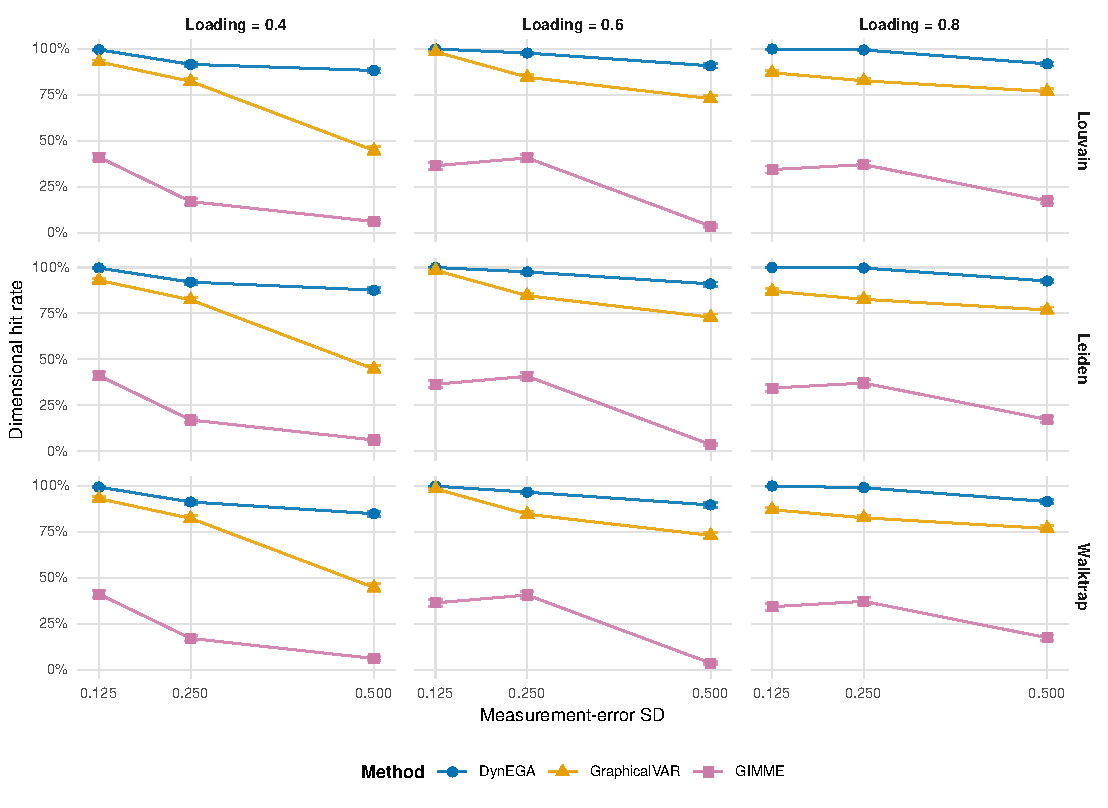
\includegraphics[width=0.95\linewidth,height=\textheight,keepaspectratio]{figures/figure6_factor_effects.pdf}

}

\caption{\label{fig-factor-effects}Paired change in overall
correct-dimension recovery under each one-at-a-time sensitivity
condition. Negative values indicate lower recovery than in the reference
condition. Error bars are 95\% bootstrap intervals from resampling whole
datasets.}

\end{figure}%

Table B2 gives the dynamic parameters used in these scenarios. Table C5
summarizes the amplitudes generated in the amplifying families E and F.
Table C6 describes deterministic growth or decay for each distinct
parameter pair. Together, these diagnostics distinguish the specified
dynamic regime from the amplitudes observed in finite simulated records.

\begingroup\scriptsize\setlength{\tabcolsep}{2pt}

\begin{longtable}[t]{crrrp{0.85in}p{0.95in}p{0.85in}p{0.85in}}
\caption{Realized amplitude diagnostics for the amplifying families E and F (Table B1) with $N=50$, four indicators per dimension, loading 0.60, residual standard deviation 0.25, and 25 replications. The final-tenth energy fraction is the proportion of squared activity-scaled latent signal occurring in the last 10\% of observations, averaged across clips within a panel and then summarized across replications.}\\
\toprule
Code & Dimensions & $T$ & $H$ & Median max $|\tilde{x}|$ & 95th percentile max $|\tilde{x}|$ & Median observed IQR & Final-tenth energy fraction\\
\midrule
\endfirsthead
\toprule
Code & Dimensions & $T$ & $H$ & Median max $|\tilde{x}|$ & 95th percentile max $|\tilde{x}|$ & Median observed IQR & Final-tenth energy fraction\\
\midrule
\endhead
E & 2 & 100 & 39.60 & 55.9 & 61.5 & 3.47 & 0.316\\
E & 2 & 300 & 74.75 & 329.4 & 376.9 & 7.46 & 0.338\\
E & 3 & 100 & 39.60 & 62.6 & 73.0 & 1.90 & 0.368\\
E & 3 & 300 & 74.75 & 430.3 & 478.6 & 4.58 & 0.428\\
E & 4 & 100 & 39.60 & 85.6 & 102.7 & 1.57 & 0.404\\
\addlinespace
E & 4 & 300 & 74.75 & 994.9 & 1092.7 & 4.02 & 0.498\\
F & 2 & 100 & 39.60 & 69.5 & 81.9 & 4.71 & 0.319\\
F & 2 & 300 & 74.75 & 388.1 & 491.3 & 9.31 & 0.324\\
F & 3 & 100 & 39.60 & 77.7 & 87.5 & 2.33 & 0.367\\
F & 3 & 300 & 74.75 & 518.5 & 608.5 & 5.74 & 0.448\\
\addlinespace
F & 4 & 100 & 39.60 & 105.2 & 122.2 & 1.92 & 0.402\\
F & 4 & 300 & 74.75 & 1201.6 & 1350.2 & 4.97 & 0.517\\
\bottomrule
\end{longtable}
\endgroup

\begin{landscape}\footnotesize\setlength{\tabcolsep}{3pt}

\begin{longtable}[t]{lrrrrrrrrp{1.30in}}
\caption{Deterministic stability diagnostics for the unique dynamic-parameter pairs used across scenario factors. Table B2 maps these pairs to scenarios and dimensions. The spectral radius $\rho(\Phi)$ is the largest absolute eigenvalue of the transition matrix; values below one indicate decay. The modal exponential-rate factors $g(H)=\exp\{H\max\operatorname{Re}(r)\}$ describe modal rates over the observed horizon rather than total finite-horizon state amplification. $H[100]=39.6$ and $H[300]=74.75$ under the stated record designs.}\\
\toprule
Scenario codes & eta & zeta & Discriminant & Max Re(root) & rho(Phi[.4]) & rho(Phi[.25]) & g(H[100]) & g(H[300]) & Regime\\
\midrule
\endfirsthead
\toprule
Scenario codes & eta & zeta & Discriminant & Max Re(root) & rho(Phi[.4]) & rho(Phi[.25]) & g(H[100]) & g(H[300]) & Regime\\
\midrule
\endhead
A, B, C, D & -1.10 & -0.30 & -4.3100 & -0.150 & 0.9418 & 0.9632 & 0.0026 & 0.0000 & Stable oscillatory\\
A, B, C, D & -0.85 & -0.65 & -2.9775 & -0.325 & 0.8781 & 0.9220 & 0.0000 & 0.0000 & Stable oscillatory\\
A, B, C, D & -0.55 & -1.00 & -1.2000 & -0.500 & 0.8187 & 0.8825 & 0.0000 & 0.0000 & Stable oscillatory\\
A, B, C, D & -0.30 & -1.70 & 1.6900 & -0.200 & 0.9231 & 0.9512 & 0.0004 & 0.0000 & Stable nonoscillatory\\
E, F & -0.20 & 0.14 & -0.7804 & 0.070 & 1.0284 & 1.0177 & 15.9906 & 187.2604 & Finite-horizon amplifying oscillatory\\
\addlinespace
E, F & -0.15 & 0.12 & -0.5856 & 0.060 & 1.0243 & 1.0151 & 10.7618 & 88.6770 & Finite-horizon amplifying oscillatory\\
E, F & -0.10 & 0.10 & -0.3900 & 0.050 & 1.0202 & 1.0126 & 7.2427 & 41.9929 & Finite-horizon amplifying oscillatory\\
E, F & -0.05 & 0.08 & -0.1936 & 0.040 & 1.0161 & 1.0101 & 4.8744 & 19.8857 & Finite-horizon amplifying oscillatory\\
\bottomrule
\end{longtable}
\end{landscape}

\newpage

\subsection{C.4 Extended Factorial
Simulation}\label{c.4-extended-factorial-simulation}

The extended factorial simulation evaluated DynEGA on 518,400 datasets.
It recovered the correct dimension in 93.7\% of those datasets and
assigned 95.2\% of indicators correctly. Stronger loadings and smaller
residual error improved recovery. The design, including the \(T=300\)
change in observation interval, is given in Appendix B. Runtime
accounting for this design is in Section C.5.

\subsection{C.5 Runtime and Feasibility
Accounting}\label{c.5-runtime-and-feasibility-accounting}

\begin{figure}[H]

\centering{

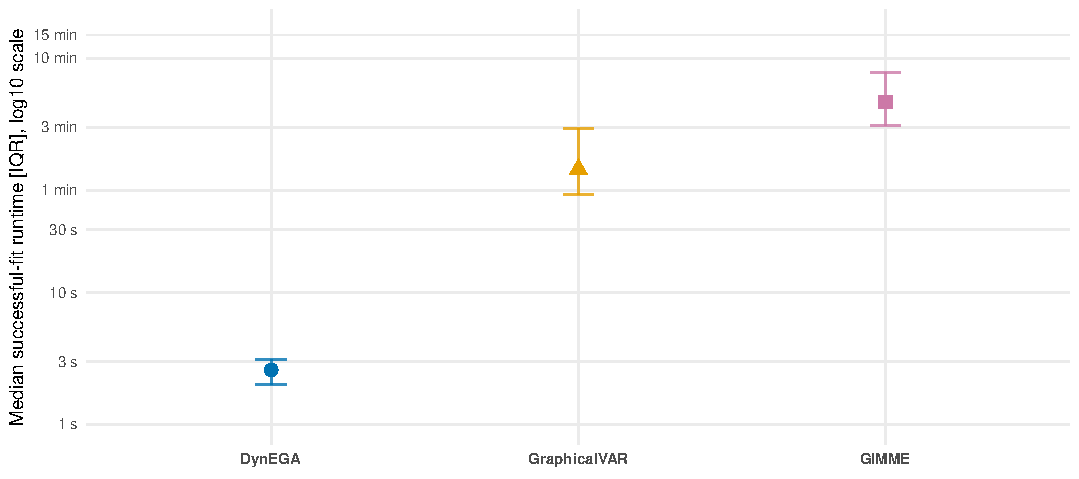
\includegraphics[width=0.95\linewidth,height=\textheight,keepaspectratio]{figures/figure7_runtime_feasibility.pdf}

}

\caption{\label{fig-runtime-feasibility}Runtime among valid network
outputs in the primary \(T=100\) and shorter \(T=25\) designs. Points
show medians and intervals show interquartile ranges on a log10 scale.
Counts use unique fitted structures.}

\end{figure}%

\begin{landscape}\footnotesize\setlength{\tabcolsep}{3pt}

\begin{longtable}[t]{lclrrrrcc}
\caption{Runtime and feasibility per method fit in the $T=100$ primary and $T=25$ shorter-series matched-method designs. Valid-output intervals resample whole simulated datasets. Runtime summaries condition on valid network outputs and include structure estimation, network extraction, and community detection. Each fitted structure is reused for Louvain, Leiden, and Walktrap.}\\
\toprule
Analysis & $T$ & Method & Attempts & Valid outputs & Timeouts & Errors & Valid-output rate & Runtime median [IQR], s\\
\midrule
\endfirsthead
\toprule
Analysis & $T$ & Method & Attempts & Valid outputs & Timeouts & Errors & Valid-output rate & Runtime median [IQR], s\\
\midrule
\endhead
Matched methods & $T=100$ & DynEGA & 21600 & 21600 & 0 & 0 & 1.000 [1.000, 1.000] & 3.69 [3.18, 4.25]\\
Matched methods & $T=100$ & GIMME & 21600 & 4846 & 14477 & 2277 & 0.224 [0.219, 0.230] & 518.16 [398.98, 603.71]\\
Matched methods & $T=100$ & GraphicalVAR & 21600 & 20329 & 1271 & 0 & 0.941 [0.938, 0.944] & 85.41 [53.82, 185.91]\\
Matched methods & $T=100$ & Static EGA & 21600 & 21526 & 0 & 74 & 0.997 [0.996, 0.997] & 2.15 [2.05, 2.26]\\
Matched methods & $T=25$ & DynEGA & 21600 & 21600 & 0 & 0 & 1.000 [1.000, 1.000] & 2.28 [2.13, 2.52]\\
\addlinespace
Matched methods & $T=25$ & GIMME & 21600 & 0 & 0 & 21600 & 0.000 [0.000, 0.000] & Not available\\
Matched methods & $T=25$ & GraphicalVAR & 21600 & 21579 & 21 & 0 & 0.999 [0.999, 0.999] & 66.49 [33.96, 169.39]\\
Matched methods & $T=25$ & Static EGA & 21600 & 21541 & 0 & 59 & 0.997 [0.997, 0.998] & 2.20 [2.10, 2.32]\\
\bottomrule
\end{longtable}
\end{landscape}

\newpage

\subsection{C.6 Community-Detection
Sensitivity}\label{c.6-community-detection-sensitivity}

Louvain, Leiden, and Walktrap were applied to each retained fitted
graph. Their results were closely aligned in the matched-method
simulation designs (Figure~\ref{fig-community-sensitivity}) and led to
the same interpretation of the one-at-a-time sensitivity conditions
(Figure~\ref{fig-challenge-community-sensitivity}). These comparisons
reuse fitted structures and therefore assess the community-detection
step rather than estimator variability.

\begin{figure}[H]

\centering{

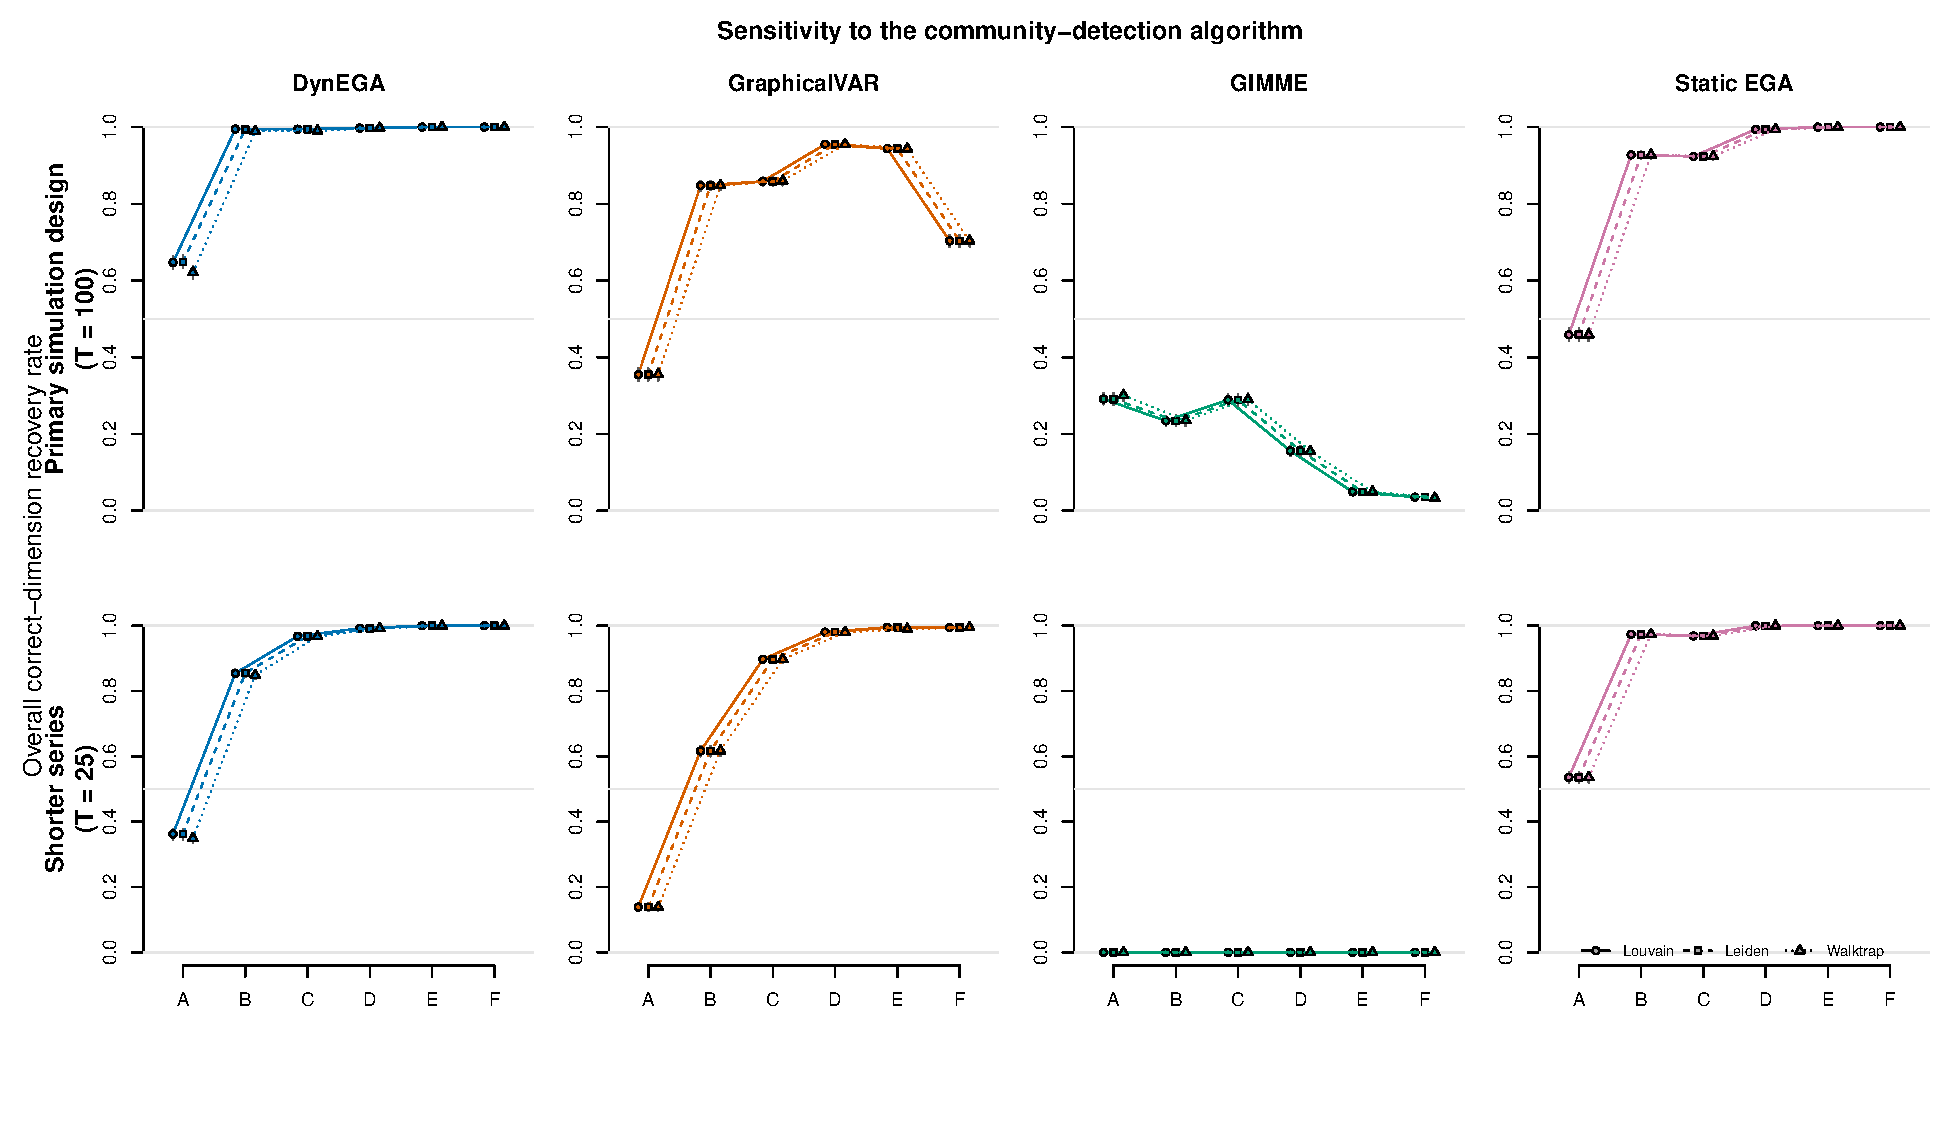
\includegraphics[width=0.98\linewidth,height=\textheight,keepaspectratio]{figures/figureS1_dimension_recovery_readout_sensitivity.pdf}

}

\caption{\label{fig-community-sensitivity}Overall correct-dimension
recovery rates for Louvain, Leiden, and Walktrap in the \(T=100\)
primary and \(T=25\) shorter-series matched-method designs. Each fitted
network is reused across all three algorithms, so differences isolate
the community-detection step.}

\end{figure}%

\begin{figure}[H]

\centering{

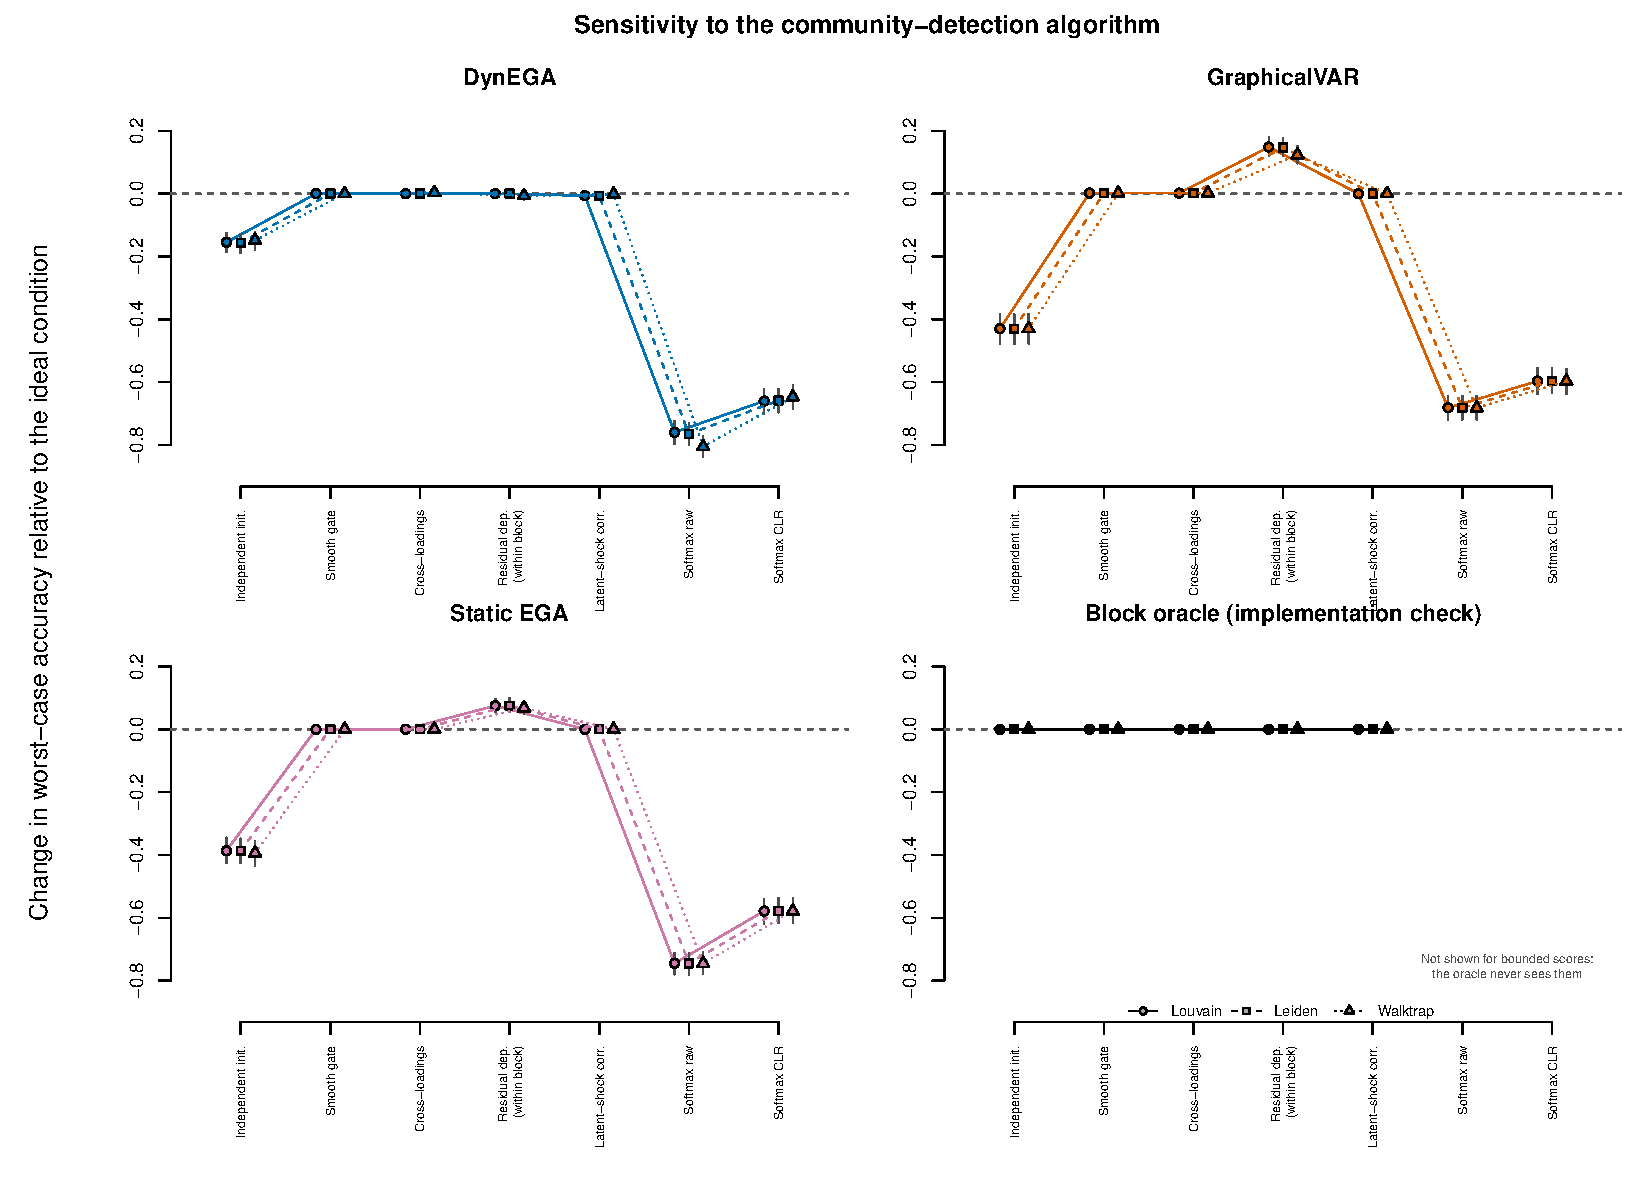
\includegraphics[width=0.98\linewidth,height=\textheight,keepaspectratio]{figures/figureS2_factor_effects_readout_sensitivity.pdf}

}

\caption{\label{fig-challenge-community-sensitivity}Sensitivity of the
paired one-at-a-time effects to Louvain, Leiden, and Walktrap. Values
are changes in overall correct-dimension recovery rate relative to the
reference condition.}

\end{figure}%

\section{References}\label{references}

\begingroup
\setlength{\parindent}{-0.5in}
\setlength{\leftskip}{0.5in}

\phantomsection\label{refs}
\begin{CSLReferences}{1}{0}
\bibitem[\citeproctext]{ref-blondel2008fast}
Blondel, V. D., Guillaume, J.-L., Lambiotte, R., \& Lefebvre, E. (2008).
Fast unfolding of communities in large networks. \emph{Journal of
Statistical Mechanics: Theory and Experiment}, \emph{2008}(10), P10008.
\url{https://doi.org/10.1088/1742-5468/2008/10/P10008}

\bibitem[\citeproctext]{ref-glla2010}
Boker, S. M., Deboek, P. R., Edler, C., \& Keel, P. (2010). Generalized
local linear approximation of derivatives from time series. In S. M.
Chow, E. Ferrer, \& F. Hsieh (Eds.), \emph{The notre dame series on
quantitative methodology. Statistical methods for modeling human
dynamics: An interdisciplinary dialogue} (pp. 161--178).
Routledge/Taylor \& Francis Group.

\bibitem[\citeproctext]{ref-graphicalVAR2024}
Epskamp, S. (2024). \emph{graphicalVAR: Graphical VAR for experience
sampling data}. \url{https://CRAN.R-project.org/package=graphicalVAR}

\bibitem[\citeproctext]{ref-epskampggm}
Epskamp, S., Waldorp, L. J., Mõttus, R., \& Borsboom, D. (2018). The
gaussian graphical model in cross-sectional and time-series data.
\emph{Multivariate Behavioral Research}, \emph{53}(4), 453--480.
\url{https://doi.org/10.1080/00273171.2018.1454823}

\bibitem[\citeproctext]{ref-gates2012group}
Gates, K. M., \& Molenaar, P. C. M. (2012). Group search algorithm
recovers effective connectivity maps for individuals in homogeneous and
heterogeneous samples. \emph{NeuroImage}, \emph{63}(1), 310--319.
\url{https://doi.org/10.1016/j.neuroimage.2012.06.026}

\bibitem[\citeproctext]{ref-golino2017ega1}
Golino, H. F., \& Epskamp, S. (2017). Exploratory graph analysis: A new
approach for estimating the number of dimensions in psychological
research. \emph{PloS One}, \emph{12}(6), e0174035.
\url{https://doi.org/10.1371/journal.pone.0174035}

\bibitem[\citeproctext]{ref-golino2020modeling}
Golino, H., Christensen, A. P., Moulder, R., Kim, S., \& Boker, S. M.
(2022). Modeling latent topics in social media using dynamic exploratory
graph analysis: The case of the right-wing and left-wing trolls in the
2016 US elections. \emph{Psychometrika}, \emph{87}(1), 156--187.

\bibitem[\citeproctext]{ref-golino2019investigating}
Golino, H., Shi, D., Garrido, L. E., Christensen, A. P., Nieto, M. D.,
Sadana, R., Thiyagarajan, J. A., \& Martinez-Molina, A. (2020).
Investigating the performance of exploratory graph analysis and
traditional techniques to identify the number of latent factors: A
simulation and tutorial. \emph{Psychological Methods}, \emph{25}(3),
292--320. \url{https://doi.org/10.1037/met0000255}

\bibitem[\citeproctext]{ref-lane2019uncovering}
Lane, S. T., Gates, K. M., Pike, H. K., Beltz, A. M., \& Wright, A. G.
C. (2019). Uncovering general, shared, and unique temporal patterns in
ambulatory assessment data. \emph{Psychological Methods}, \emph{24}(1),
54--69. \url{https://doi.org/10.1037/met0000192}

\bibitem[\citeproctext]{ref-pons2006walktrap}
Pons, P., \& Latapy, M. (2005). Computing communities in large networks
using random walks. In Pi. Yolum, T. Güngör, F. Gürgen, \& C. Özturan
(Eds.), \emph{Computer and information sciences - ISCIS 2005} (pp.
284--293). Springer Berlin Heidelberg.
\url{https://doi.org/10.1007/11569596_31}

\bibitem[\citeproctext]{ref-traag2019leiden}
Traag, V. A., Waltman, L., \& Eck, N. J. van. (2019). From louvain to
leiden: Guaranteeing well-connected communities. \emph{Scientific
Reports}, \emph{9}(1), 5233.
\url{https://doi.org/10.1038/s41598-019-41695-z}

\end{CSLReferences}

\endgroup




\end{document}
